\chapter{Anillos conmutativos}

En este capítulo vamos a ver algunas nociones básicas
del \term{álgebra conmutativa}, la rama de álgebra que se dedica al estudio
de anillos conmutativos.

% % % % % % % % % % % % % % % % % % % % % % % % % % % % % %

\section{Ideales primos y maximales}

\begin{definicion}
  \label{dfn:ideales-primos-y-maximales}
  Sea $R$ un anillo conmutativo.

  Se dice que un ideal $\mathfrak{p} \subset R$ es
  \term{primo}\index{ideal!primo} si se cumplen las siguientes condiciones:

  \begin{enumerate}
  \item[1)] $\mathfrak{p}$ es un ideal propio: $\mathfrak{p} \ne R$,

  \item[2)] para cualesquiera $x,y\in R$ si $xy \in \mathfrak{p}$, entonces
    $x \in \mathfrak{p}$ o $y \in \mathfrak{p}$.
  \end{enumerate}

  Se dice que un ideal $\mathfrak{m} \subset R$ es
  \term{maximal}\index{ideal!maximal} si se cumplen las siguientes condiciones:

  \begin{enumerate}
  \item[1)] $\mathfrak{m}$ es un ideal propio: $\mathfrak{m} \ne R$,

  \item[2)] $\mathfrak{m}$ es \term{maximal} respecto a la inclusión: para todo
    ideal $I \subseteq R$ tal que $\mathfrak{m} \subseteq I \subseteq R$ se
    cumple $I = \mathfrak{m}$ o $I = R$.
  \end{enumerate}
\end{definicion}

\begin{comentario}
  Las letras $\mathfrak{p}$ y $\mathfrak{m}$ son $p$ y $m$ \emph{góticas}. Esta
  notación es común en álgebra conmutativa y viene de la tradición alemana.
\end{comentario}

\begin{notacion}
  Sea $R$ un anillo conmutativo. El conjunto de los ideales primos en $R$
  se llama el \term{espectro}\index{espectro!de anillo conmutativo} de $R$
  y se denota por $\Spec R$\index[notacion]{Spec R@$\Spec R$}:
  \[ \Spec R \dfn \{ \mathfrak{p} \subset R \mid
                     \mathfrak{p}\text{ ideal primo} \}. \]
  El conjunto de los ideales maximales se llama el \term{espectro
    maximal}\index{espectro!maximal} y lo vamos a denotar por\footnote{A
    diferencia de $\Spec R$, esta notación no es estándar. En la literatura
    también aparece $\operatorname{Spec-max} R$ y $\operatorname{Max} R$.}
  \[ \Specm R \dfn \{ \mathfrak{m} \subset R \mid
                     \mathfrak{m}\text{ ideal maximal} \}. \]
\end{notacion}

\begin{ejemplo}
  El anillo nulo $0$ no tiene ideales propios y entonces
  $\Spec 0 = \Specm 0 = \emptyset$. Más adelante vamos a ver que si $R \ne 0$,
  entonces $\Spec R \ne \emptyset$ y $\Specm R \ne \emptyset$.
\end{ejemplo}

\begin{ejemplo}
  En el anillo $\ZZ$ los ideales son de la forma $n\ZZ$ para
  $n = 0,1,2,3,\ldots$ Tenemos $x \in n\ZZ$ si y solamente si $n \mid x$.
  Luego, $n\ZZ$ es un ideal primo si
  \begin{enumerate}
  \item[1)] $n \ne 1$,
  \item[2)] para cualesquiera $x,y\in\ZZ$ si $n \mid xy$, entonces $n \mid x$ o
    $n \mid y$.
  \end{enumerate}

  Estas condiciones se cumplen para $n = 0$. Si $n \ne 0$, estas condiciones se
  cumplen si y solo si $n = p$ es un número primo. Entonces,
  $$\Spec \ZZ = \{ 0 \} \cup \{ p\ZZ \mid p\text{ primo} \}.$$

  Un ideal $n\ZZ$ es maximal si
  \begin{enumerate}
  \item[1)] $n \ne 1$,
  \item[2)] para todo ideal $m\ZZ \subseteq \ZZ$ tal que
    $n\ZZ \subseteq m\ZZ \subseteq \ZZ$ se cumple $n\ZZ = m\ZZ$ o $m\ZZ = \ZZ$.
  \end{enumerate}

  Recordamos que $n\ZZ \subseteq m\ZZ$ si y solo si $m\mid n$. Entonces,
  la condición 2) dice que si $m\mid n$, entonces $m = n$ o $m = 1$.
  Esto significa precisamente que $n = p$ es un número primo. Entonces,
  \[ \Specm \ZZ = \{ p\ZZ \mid p\text{ primo} \}. \qedhere \]
\end{ejemplo}

En particular, este ejemplo demuestra que los ideales primos generalizan
la noción de números primos. Tenemos la siguiente caracterización de ideales
primos.

\begin{proposicion}
  Sea $R$ un anillo conmutativo. Las siguientes condiciones son equivalentes:

  \begin{enumerate}
  \item[1)] $\mathfrak{p} \subset R$ es un ideal primo,

  \item[2)] el anillo cociente $R/\mathfrak{p}$ es un dominio de integridad.
  \end{enumerate}

  \begin{proof}
    Por la definición, $\mathfrak{p} \subset R$ es un ideal primo si y solo si
    1) $\mathfrak{p} \ne R$ y 2) $xy \in \mathfrak{p}$ implica
    $x\in \mathfrak{p}$ o $y\in \mathfrak{p}$. En términos del anillo cociente
    $R/\mathfrak{p}$, esto es equivalente a
    \begin{enumerate}
    \item[1)] $R/\mathfrak{p} \ne 0$,

    \item[2)] si
      $(x + \mathfrak{p})\,(y + \mathfrak{p}) \dfn xy + \mathfrak{p} =
      \overline{0}$\footnote{Aquí $\overline{0}$ denota la clase lateral
        $0 + \mathfrak{p}$ en el cociente $R/\mathfrak{p}$.}, entonces
      $x + \mathfrak{p} = \overline{0}$ o $y + \mathfrak{p} = \overline{0}$.
    \end{enumerate}

    En otras palabras, $R/\mathfrak{p}$ es un anillo conmutativo no nulo que no
    tiene divisores de cero. Es precisamente la definición de dominio de
    integridad.
  \end{proof}
\end{proposicion}

Los ideales maximales tienen una caracterización parecida.

\begin{proposicion}
  Sea $R$ un anillo conmutativo. Las siguientes condiciones son equivalentes:
  \begin{enumerate}
  \item[1)] $\mathfrak{m} \subset R$ es un ideal maximal,

  \item[2)] el anillo cociente $R/\mathfrak{m}$ es un cuerpo.
  \end{enumerate}

  \begin{proof}
    Recordemos que un anillo conmutativo $S$ es un cuerpo si y solo si sus
    únicos ideales son $0$ y $S$. Además, tenemos la siguiente descripción
    de los ideales en el anillo cociente $R/\mathfrak{m}$:

    \begin{align*}
      \{ \text{ideales }\overline{I} \subseteq R/\mathfrak{m} \} &
      \xrightarrow{\isom}
      \{ \text{ideales }\mathfrak{m} \subseteq I \subseteq R \},\\
      \overline{I} & \mapsto \pi^{-1} (\overline{I}),
    \end{align*}
    donde $\pi\colon R\to R/\mathfrak{m}$ denota la proyección canónica
    $x \mapsto x + \mathfrak{m}$.

    En particular, los ideales $\overline{0}$ y $R/\mathfrak{m}$ en el cociente
    corresponden a los ideales $I = \mathfrak{m}$ e $I = R$ en $R$. El anillo
    $R/\mathfrak{m}$ no tiene otros ideales si y solamente si
    $\mathfrak{m} \subseteq I \subseteq R$ implica $I = \mathfrak{m}$ o
    $I = R$. Esta es precisamente la condición de la definición de ideales
    maximales.
  \end{proof}
\end{proposicion}

\begin{ejemplo}
  El anillo cociente $\ZZ/n\ZZ$ es un dominio de integridad si y solo si $n = 0$
  o $n = p$ es un número primo y es un cuerpo si y solo si $n = p$.
  Esto coincide con nuestra descripción de los ideales primos y maximales en
  $\ZZ$.

  \begin{center}
    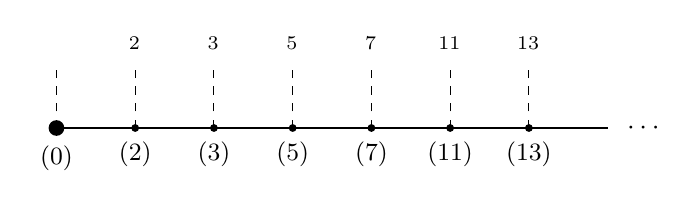
\begin{tikzpicture}
      \draw (0,0) node[label=left:{$\Spec \ZZ$}] {};

      \draw (0,0) node[circle,fill,inner sep=2pt, label=below:{\small $(0)$}] {};
      \draw (1,0) node[circle,fill,inner sep=1pt, label=below:{\small $(2)$}] {};
      \draw (2,0) node[circle,fill,inner sep=1pt, label=below:{\small $(3)$}] {};
      \draw (3,0) node[circle,fill,inner sep=1pt, label=below:{\small $(5)$}] {};
      \draw (4,0) node[circle,fill,inner sep=1pt, label=below:{\small $(7)$}] {};
      \draw (5,0) node[circle,fill,inner sep=1pt, label=below:{\small $(11)$}] {};
      \draw (6,0) node[circle,fill,inner sep=1pt, label=below:{\small $(13)$}] {};

      \draw (7,0) node[label=right:{$\cdots$}] {};

      \draw[dashed] (0,0) -- (0,0.75) node[label=above:{$\ZZ$}] {};
      \draw[dashed] (1,0) -- (1,0.75) node[label=above:{$\FF_2$}] {};
      \draw[dashed] (2,0) -- (2,0.75) node[label=above:{$\FF_3$}] {};
      \draw[dashed] (3,0) -- (3,0.75) node[label=above:{$\FF_5$}] {};
      \draw[dashed] (4,0) -- (4,0.75) node[label=above:{$\FF_7$}] {};
      \draw[dashed] (5,0) -- (5,0.75) node[label=above:{$\FF_{11}$}] {};
      \draw[dashed] (6,0) -- (6,0.75) node[label=above:{$\FF_{13}$}] {};

      \draw (0,0) -- (7,0);
    \end{tikzpicture}

    El espectro de $R = \ZZ$ con los anillos cociente correspondientes
    $R/\mathfrak{p}$
  \end{center}
\end{ejemplo}

\begin{corolario}
  Sea $R$ un anillo conmutativo. Todo ideal maximal $\mathfrak{m} \subset R$ es
  un ideal primo.

  \begin{proof}
    Si $R/\mathfrak{m}$ es un cuerpo, en particular es un dominio de integridad.
  \end{proof}
\end{corolario}

\begin{corolario}
  Sea $R$ un anillo conmutativo.

  \begin{enumerate}
  \item[1)] El ideal nulo $0$ es primo en $R$ si y solo si $R$ es un dominio
    de integridad,

  \item[2)] El ideal nulo $0$ es maximal en $R$ si y solo si $R$ es un cuerpo.
  \end{enumerate}

  \begin{proof}
    $R/0 \isom R$.
  \end{proof}
\end{corolario}

\begin{observacion}
  \label{obs:preimagen-de-un-ideal-primo}
  Sea $f\colon R\to S$ un homomorfismo de anillos conmutativos.

  \begin{enumerate}
  \item[1)] Si $\mathfrak{p} \subset S$ es un ideal primo, entonces
    $f^{-1} (\mathfrak{p})$ es un ideal primo en $R$. En otras palabras,
    un homomorfismo de anillos $f\colon R\to S$ induce una aplicación entre los
    espectros
    $$\Spec S \to \Spec R, \quad \mathfrak{p} \mapsto f^{-1} (\mathfrak{p}).$$

  \item[2)] Si $f$ es sobreyectivo y $\mathfrak{m} \subset S$ es un ideal
    maximal, entonces $f^{-1} (\mathfrak{m})$ es un ideal maximal en $R$.
  \end{enumerate}

  \begin{proof}
    Para un ideal $I \subseteq S$ podemos considerar el homomorfismo
    $$R \xrightarrow{f} S \xrightarrow{\pi} S/I$$
    donde $\pi\colon s \mapsto s + I$ es la proyección sobre el anillo
    cociente. Tenemos
    $$\ker (\pi\circ f) = \{ r \in R \mid f (r) \in I \} = f^{-1} (I).$$
    Luego, el primer teorema de isomorfía implica que
    $$R/f^{-1} (I) \isom \im (\pi\circ f) \subseteq S/I.$$

    Ahora en la parte 1), si $I = \mathfrak{p}$ es un ideal primo, entonces
    $S/\mathfrak{p}$ es un dominio de integridad, y luego
    $\im (\pi\circ f) \isom R/f^{-1} (\mathfrak{p})$ es también un dominio de
    integridad, siendo un subanillo. Esto implica que $f^{-1} (\mathfrak{p})$ es
    un ideal primo en $R$.

    En la parte 2), si $f$ es un homomorfismo sobreyectivo, entonces
    $\im (\pi\circ f) = S/I$. Si $I = \mathfrak{m}$ es un ideal maximal,
    entonces $S/\mathfrak{m}$ es un cuerpo, y luego
    $S/\mathfrak{m} \isom R/f^{-1} (\mathfrak{m})$ es también un cuerpo y por lo
    tanto el ideal $f^{-1} (\mathfrak{m})$ es maximal en $R$.
  \end{proof}
\end{observacion}

\begin{comentario}
  En general, para un homomorfismo de anillos $f\colon R\to S$,
  si $\mathfrak{m} \subset S$ es un ideal maximal, entonces
  $f^{-1} (\mathfrak{m})$ no tiene por qué ser un ideal maximal en
  $R$. Considere por ejemplo la inclusión $f\colon \ZZ \hookrightarrow \QQ$.
  El ideal nulo $0$ es maximal en $\QQ$, pero $0 = f^{-1} (0)$ no es un ideal
  maximal en $\ZZ$. En este sentido los ideales primos se comportan mejor que
  los maximales.
\end{comentario}

\begin{proposicion}
  \label{prop:ideales-primos-y-maximales-en-el-cociente}
  Sean $R$ un anillo conmutativo, $I \subseteq R$ un ideal y
  $\pi\colon R\to R/I$ la proyección correspondiente sobre el anillo
  cociente. La biyección
  \begin{align*}
    \{ \text{ideales }\overline{J} \subseteq R/I \} & \leftrightarrow
    \{ \text{ideales }I \subseteq J \subseteq R \},\\
    \overline{J} & \mapsto \pi^{-1} (\overline{J}),\\
    J & \mapsfrom J/I
  \end{align*}
  se restringe a las biyecciones
  \begin{align*}
    \Spec R/I & \leftrightarrow
    \{ \mathfrak{p} \in \Spec R \mid I \subseteq \mathfrak{p} \},\\
    \Specm R/I & \leftrightarrow
    \{ \mathfrak{m} \in \Specm R \mid I \subseteq \mathfrak{m} \}.
  \end{align*}

  \begin{proof}
    Para los ideales primos, ya vimos en \ref{obs:preimagen-de-un-ideal-primo}
    que si $\overline{\mathfrak{p}} \subset R/I$ es un ideal primo, entonces
    $\pi^{-1} (\overline{\mathfrak{p}}) \subset R$ es un ideal primo. Además,
    notamos que para un ideal primo $I \subseteq \mathfrak{p} \subset R$ el
    ideal $\mathfrak{p}/I \subset R/I$ es también primo. En efecto,
    \[ \mathfrak{p} \text{ es primo} \iff
       R/\mathfrak{p} \text{ es un dominio}; \quad
       \mathfrak{p}/I \text{ es primo} \iff
       (R/I)/(\mathfrak{p}/I) \text{ es un dominio}, \]
    pero según el tercer teorema de isomorfía,
    $$(R/I)/(\mathfrak{p}/I) \isom R/\mathfrak{p}.$$
    De la misma manera, si $\overline{\mathfrak{m}} \subset R/I$ es un ideal
    maximal, entonces $\pi^{-1} (\overline{\mathfrak{m}})$ es un ideal maximal
    en $R$ como notamos en \ref{obs:preimagen-de-un-ideal-primo} (usando que
    $\pi\colon R\to R/I$ es un homomorfismo sobreyectivo). Luego, para un ideal
    $I \subseteq \mathfrak{m} \subseteq R$ tenemos
    \[ \mathfrak{m} \text{ es maximal} \iff
       R/\mathfrak{m} \text{ es un cuerpo};
       \quad
       \mathfrak{m}/I \text{ es maximal} \iff
       (R/I)/(\mathfrak{m}/I) \text{ es un cuerpo}, \]
    y de nuevo, es suficiente aplicar el tercer teorema de isomorfía
    \[ (R/I)/(\mathfrak{m}/I) \isom R/\mathfrak{m}. \qedhere \]
  \end{proof}
\end{proposicion}

El siguiente resultado establece la existencia de ideales maximales.

\begin{proposicion}
  \label{prop:existencia-de-ideales-maximales}
  Todo anillo conmutativo no nulo posee un ideal maximal.
\end{proposicion}

Para probarlo, necesitamos el lema de Zorn. El lector puede consultar
el apéndice B para revisar el enunciado.

\begin{proof}[Demostración de \ref{prop:existencia-de-ideales-maximales}]
  Sea $R$ un anillo conmutativo no nulo y sea $\mathcal{P}$ el conjunto de los
  ideales propios $I \subsetneq R$. Esto es un conjunto parcialmente ordenado
  respecto a la inclusión $I \subseteq J$. Por la hipótesis, $R \ne 0$, así que
  $0 \in \mathcal{P}$ y por lo tanto $\mathcal{P} \ne \emptyset$. Un elemento
  maximal en $\mathcal{P}$ sería precisamente un ideal maximal en $R$. Para
  deducir la existencia de un elemento maximal, tenemos que probar que toda
  cadena en $\mathcal{P}$ es acotada.

  Una cadena en $\mathcal{P}$ es una colección de ideales propios
  $\mathcal{S} = \{ I_\alpha \}$ donde $I_\alpha \subseteq I_\beta$ o
  $I_\beta \subseteq I_\alpha$ para cualesquiera $\alpha, \beta$. Se ve que la
  unión $I \dfn \bigcup_\alpha I_\alpha$ es también un ideal en $R$\footnote{De
    hecho, $0 \in I_\alpha$ para todo $\alpha$, así que $0 \in I$. Para
    $x,y \in I$ tenemos $x\in I_\alpha$ e $y\in I_\beta$ para algunos
    $\alpha,\beta$. Sin pérdida de generalidad, $I_\alpha \subseteq I_\beta$,
    así que $x+y \in I_\beta$, dado que $I_\beta$ es un ideal. Para todo
    $r\in R$ y $x \in I$ se tiene $x \in I_\alpha$ para algún $\alpha$, y luego
    $rx \in I_\alpha \subseteq I$.}. Dado que $1 \notin I_\alpha$ para todo
  $\alpha$, tenemos $1\notin I$, así que $I$ es también un ideal propio e
  $I \in \mathcal{P}$. Tenemos $I_\alpha \subseteq I$ para todo $\alpha$. Este
  ideal $I$ es una cota superior para $\mathcal{S}$.
\end{proof}

\begin{corolario}
  Sea $R$ un anillo conmutativo y sea $I \subsetneq R$ un ideal
  propio. Entonces, $R$ posee un ideal maximal $\mathfrak{m} \subset R$ tal que
  $I \subseteq \mathfrak{m}$.

  \begin{proof}
    Si $I \ne R$, entonces el anillo $R/I$ no es nulo y según
    \ref{prop:existencia-de-ideales-maximales} posee un ideal maximal
    $\overline{\mathfrak{m}} \subset R/I$. Luego, como vimos en
    \ref{prop:ideales-primos-y-maximales-en-el-cociente}, este ideal corresponde
    a un ideal maximal
    $\mathfrak{m} = \pi^{-1} (\overline{\mathfrak{m}}) \subset R$ tal que
    $I \subseteq \mathfrak{m}$.
  \end{proof}
\end{corolario}

He aquí otro resultado importante sobre los ideales que puede ser demostrado
mediante el lema de Zorn.

\begin{proposicion}
  Sea $R$ un anillo conmutativo. Entonces, su nilradical coincide con
  la intersección de los ideales primos en $R$:
  \[ N (R) \dfn \{ r \in R \mid r^n = 0 \text{ para algún }n=1,2,3,\ldots \}
           = \bigcap_{\mathfrak{p} \in \Spec R} \mathfrak{p}. \]

  \begin{proof}
    Sea $r \in N (R)$ un nilpotente. Luego, $r^n = 0$ para algún $n$ y por ende
    $r^n \in \mathfrak{p}$ para cualquier ideal primo $\mathfrak{p} \subset R$,
    lo que implica que $r\in \mathfrak{p}$. Entonces, $r$ pertenece a cualquier
    ideal primo. Esto demuestra la inclusión
    $$N (R) \subseteq \bigcap_{\mathfrak{p} \in \Spec R} \mathfrak{p}.$$

    Para probar la otra inclusión, vamos a ver que si $r\notin N (R)$, entonces
    existe un ideal primo $\mathfrak{p} \subset R$ tal que
    $r\notin \mathfrak{p}$. Supongamos entonces que $r\in R$ satisface
    $r^n \ne 0$ para todo $n = 1,2,3,\ldots$ Sea $\mathcal{P}$ el conjunto de
    los ideales $I \subset R$ que no contienen ninguna potencia de $r$:
    \[ U \cap I = \emptyset, \quad
       \text{donde }U \dfn \{ r^n \mid n = 1,2,3,\ldots \}.\]
    Esto es un conjunto parcialmente ordenado respecto a la inclusión.
    Notamos que $0 \in \mathcal{P}$, así que $\mathcal{P} \ne \emptyset$.
    Sea $\{ I_\alpha \}$ una cadena en $\mathcal{P}$. Entonces,
    $I \dfn \bigcup_\alpha I_\alpha$ es también un ideal, como ya notamos en
    la demostración de \ref{prop:existencia-de-ideales-maximales}. Dado que
    $U \cap I_\alpha = \emptyset$ para todo $\alpha$, tenemos
    $U \cap I = \emptyset$. Esto significa que $I \in \mathcal{P}$. El ideal $I$
    es una cota superior para la cadena $\{ I_\alpha \}$. Ahora el lema de Zorn
    implica que existe un elemento maximal en $\mathcal{P}$; es decir, un ideal
    $\mathfrak{p} \subset R$ tal que\footnote{Cuidado: es un ideal maximal
      \emph{respecto a la propiedad} $U \cap I = \emptyset$, pero no es
      necesariamente un ideal maximal en el anillo $R$.}

    \begin{enumerate}
    \item[1)] $U \cap \mathfrak{p} = \emptyset$,

    \item[2)] si $I \subset R$ es otro ideal que satisface
      $U \cap I = \emptyset$ y $\mathfrak{p} \subseteq I$, entonces
      $I = \mathfrak{p}$.
    \end{enumerate}

    La notación ``$\mathfrak{p}$'' no es una coincidencia: ahora vamos a probar
    que esto es un ideal primo. Primero, $r\notin \mathfrak{p}$, así que esto es
    un ideal propio. Además, si $xy \in \mathfrak{p}$ para algunos $x,y\in R$,
    necesitamos probar que $x\in \mathfrak{p}$ o $y\in \mathfrak{p}$. Supongamos
    que $x \notin \mathfrak{p}$ e $y \notin \mathfrak{p}$ para obtener una
    contradicción. En este caso
    \[ (x) + \mathfrak{p} \supsetneq \mathfrak{p}, \quad
       (y) + \mathfrak{p} \supsetneq \mathfrak{p}, \]
    lo que implica que
    \[ U \cap ((x) + \mathfrak{p}) \ne \emptyset, \quad
       U \cap ((y) + \mathfrak{p}) \ne \emptyset; \]
    es decir, que existen algunas potencias
    \[ r^m = sx + p \in (x) + \mathfrak{p}, \quad
       r^n = ty + q \in (y) + \mathfrak{p} \]
    para algunos $m,n \ge 1$, $s,t\in R$, $p,q\in \mathfrak{p}$. Tenemos
    $$r^{m+n} = (sx + p)\,(st + q) = stxy + sxq + tyq + pq.$$
    Dado que $\mathfrak{p}$ es un ideal y $xy \in \mathfrak{p}$, este elemento
    pertenece a $\mathfrak{p}$. Sin embargo, esto contradice la propiedad que
    $U \cap \mathfrak{p} = \emptyset$. Podemos concluir que $\mathfrak{p}$ es
    un ideal primo.

    Entonces, existe un ideal primo $\mathfrak{p} \subset R$ tal que
    $U \cap \mathfrak{p} = \emptyset$, y en particular $r \notin \mathfrak{p}$.
  \end{proof}
\end{proposicion}

\begin{ejemplo}
  Los ideales en el anillo $\ZZ/12\ZZ$ corresponden a los ideales en $\ZZ$ que
  contienen a $12\ZZ$:
  $$\ZZ, ~ 2\ZZ, ~ 3\ZZ, ~ 4\ZZ, ~ 6\ZZ, ~ 12\ZZ.$$
  Los ideales primos en $\ZZ/12\ZZ$ corresponden a los ideales primos en
  la lista de arriba, así que son
  \begin{align*}
    2\ZZ/12\ZZ & = \{ [0], [2], [4], [6], [8], [10] \},\\
    3\ZZ/12\ZZ & = \{ [0], [3], [6], [9] \}.
  \end{align*}
  Su intersección es
  $$2\ZZ/12\ZZ \cap 3\ZZ/12\ZZ = 6\ZZ/12\ZZ = \{ [0], [6] \}$$
  y se ve que $[0]$ y $[6]$ son precisamente los nilpotentes en $\ZZ/12\ZZ$.
\end{ejemplo}

\begin{ejemplo}
  Si $R$ es un dominio de integridad, entonces $(0)$ es un ideal primo y
  la intersección de todos los ideales primos $\mathfrak{p} \subset R$
  es necesariamente nula. Esto coincide con el hecho de que un dominio
  de integridad no pueda tener nilpotentes.
\end{ejemplo}

\begin{corolario}
  Sea $R$ un anillo conmutativo y sea $I \subseteq R$ un ideal. Entonces,
  el radical de $I$ coincide con la intersección de todos los ideales primos
  que contienen a $I$:
  \[ \sqrt{I} \dfn \{ r\in R \mid r^n \in I \text{ para algún }n = 1,2,3,\ldots \} =
  \bigcap_{\substack{\mathfrak{p} \in \Spec R \\ I \subseteq \mathfrak{p}}} \mathfrak{p}. \]

  \begin{proof}
    Si $r^n \in I$ para algún $n$ e $I \subseteq \mathfrak{p}$ para un ideal
    primo $\mathfrak{p} \subset R$, entonces $r \in \mathfrak{p}$. Esto
    demuestra que $\sqrt{I}$ pertenece a la intersección. Viceversa, supongamos
    que $r \in \mathfrak{p}$ para todo ideal primo $\mathfrak{p}$ tal que
    $I \subseteq \mathfrak{p}$. Recordemos que los ideales primos
    $I \subseteq \mathfrak{p} \subset R$ están en biyección con los ideales
    primos en el anillo cociente $R/I$. Esta biyección implica que
    $r + I \in \overline{\mathfrak{p}}$ para todo ideal primo
    $\overline{\mathfrak{p}} \subset R/I$. Entonces,
    \[ r + I \in
       \bigcap_{\overline{\mathfrak{p}} \in \Spec R/I} \overline{\mathfrak{p}} =
       N (R/I).\]
     Pero para $r + I$ ser nilpotente en $R/I$ significa precisamente que
     $r \in \sqrt{I}$.
  \end{proof}
\end{corolario}

He aquí otra aplicación más del lema de Zorn.

\begin{teorema}[I.S. Cohen]
  Sea $R$ un anillo conmutativo. Supongamos que todo ideal primo en $R$
  es finitamente generado. Entonces, todos los ideales en $R$ son finitamente
  generados.

  \begin{proof}
    Vamos a ver que si en $R$ hay un ideal que no es finitamente generado,
    entonces en $R$ hay un ideal primo que no es finitamente generado.

    Sea $\mathcal{P}$ el conjunto de los ideales que no son finitamente
    generados, parcialmente ordenado respecto a la inclusión. Por nuestra
    hipótesis, $\mathcal{P} \ne \emptyset$. Para una cadena de tales ideales
    $\{ I_\alpha \}$ la unión $I \dfn \bigcup_\alpha I_\alpha$ es también un
    ideal y no es finitamente generado. De hecho, si $I = (x_1,\ldots,x_n)$ para
    $x_1, \ldots, x_n \in R$, entonces $x_1,\ldots,x_n \in I_\alpha$ para algún
    $\alpha$ (usando que $\{ I_\alpha \}$ es una cadena), lo que implicaría que
    el ideal $I_\alpha = I$ es finitamente generado.

    Ahora según el lema de Zorn, existe un ideal $\mathfrak{p} \subset R$ que
    es maximal respecto a la propiedad de no ser finitamente generado:

    \begin{enumerate}
    \item[1)] $\mathfrak{p}$ no es finitamente generado,

    \item[2)] si $\mathfrak{p} \subseteq I \subset R$ para otro ideal $I$ que
      no es finitamente generado, entonces $I = \mathfrak{p}$.
    \end{enumerate}

    Vamos a probar que $\mathfrak{p}$ es un ideal primo. Primero, es un ideal
    propio, puesto que $R = (1)$ es finitamente generado. Supongamos que
    $xy \in \mathfrak{p}$ para algunos $x,y\in R$, pero $x\notin \mathfrak{p}$ e
    $y\notin \mathfrak{p}$. Luego,
    $$(x) + \mathfrak{p} \supsetneq \mathfrak{p},$$
    así que $(x) + \mathfrak{p}$ es un ideal finitamente generado:
    $$(x) + \mathfrak{p} = (y_1,\ldots,y_n)$$
    para algunos $y_1,\ldots,y_n \in (x) + \mathfrak{p}$. En particular, tenemos
    $$y_i = r_i\,x + p_i$$
    para algunos $r_i\in R$, $p_i \in \mathfrak{p}$. Notamos que
    $$(x) + \mathfrak{p} = (x,p_1,\ldots,p_n).$$
    De hecho, dado que $y_i \in (x,p_1,\ldots,p_n)$ para todo $i$, se cumple
    $(y_1,\ldots,y_n) \subseteq (x,p_1,\ldots,p_n)$. Viceversa,
    $x \in (x) + \mathfrak{p}$ y
    $p_i \in \mathfrak{p} \subsetneq (x) + \mathfrak{p}$ para todo
    $i = 1,\ldots,n$, así que
    $(x,p_1,\ldots,p_n) \subseteq (x) + \mathfrak{p} = (y_1,\ldots,y_n)$.

    Para un elemento arbitrario $p \in \mathfrak{p}$ tenemos en particular
    $p\in (x) + \mathfrak{p} = (x,p_1,\ldots,p_n)$, y por ende
    \begin{equation}
      \label{eqn:cohen-expresion-para-p}
      p = r\,x + r_1\,p_1 + \cdots + r_n\,p_n
    \end{equation}
    para algunos $r, r_1,\ldots,r_n \in R$. Luego,
    $$r\,x = p - (r_1\,p_1 + \cdots + r_n\,p_n),$$
    así que
    $$r \in \{ s\in R \mid sx \in \mathfrak{p} \}.$$
    Notamos que el último conjunto es un ideal y denotémoslo por $I$.
    Tenemos $\mathfrak{p} \subsetneq I$, dado que $\mathfrak{p}$ es un ideal e
    $y \in I$, pero $y \notin \mathfrak{p}$ por nuestra hipótesis. Entonces, por
    la maximalidad de $\mathfrak{p}$, el ideal $I$ debe ser finitamente
    generado:
    $$I = (z_1,\ldots,z_k)$$
    para algunos $z_1,\ldots,z_k \in I$. Esto significa que todo elemento de
    $\mathfrak{p}$ puede ser escrito como
    $$p = (a_1\,z_1 + \cdots + a_k\,z_k)\,x + (r_1\,p_1 + \cdots + r_n\,p_n),$$
    y por ende
    $$\mathfrak{p} \subseteq (z_1 x, \ldots, z_k x, p_1, \ldots, p_n).$$
    Pero por la definición de $I$, aquí $z_i x \in \mathfrak{p}$ para todo
    $i = 1,\ldots,k$ puesto que $z_i \in I$, así que
    $$\mathfrak{p} = (z_1 x, \ldots, z_k x, p_1, \ldots, p_n).$$
    Esto contradice el hecho de que $\mathfrak{p}$ no sea finitamente
    generado. Entonces, $\mathfrak{p}$ debe ser un ideal primo.
  \end{proof}
\end{teorema}

La prueba de arriba de que $\mathfrak{p}$ sea primo usa cierto truco, pero
el argumento general es una aplicación típica del lema de Zorn.

% % % % % % % % % % % % % % % % % % % % % % % % % % % % % %

\section{Localización}

En esta sección vamos a estudiar una construcción importante para anillos
conmutativos llamada \term{localización}. La idea es bien sencilla y puede ser
motivada por la construcción de los números racionales $\QQ$ a partir de
los números enteros $\ZZ$. Los elementos de $\QQ$ son fracciones $\frac{a}{b}$,
donde $a,b\in \ZZ$ y $b\ne 0$. Tenemos
\begin{equation}
  \label{eqn:igualdad-de-fracciones}
  \frac{a}{b} = \frac{a'}{b'} \iff ab' - a'b = 0.
\end{equation}
La suma y producto de fracciones se definen mediante las fórmulas
\begin{equation}
  \label{eqn:sumas-y-productos-de-fracciones}
  \frac{a}{b} + \frac{c}{d} = \frac{ad + cb}{bd}, \quad
  \frac{a}{b}\cdot\frac{c}{d} = \frac{ac}{bd}.
\end{equation}
Notamos que si $\frac{a}{b} = \frac{a'}{b'}$, entonces
\[ \frac{ad + cb}{bd} =
   \frac{a}{b} + \frac{c}{d} =
   \frac{a'}{b'} + \frac{c}{d} =
   \frac{a'd + cb'}{b'd}. \]
En efecto,
\[ (ad + cb)\,b'd - (a'd + cb')\,bd =
   ab'd^2 + \cancel{cbb'd} - a'bd^2 - \cancel{cb'bd} =
   d^2\,(\underbrace{ab' - a'b}_{= 0}) = 0. \]
De la misma manera, si $\frac{a}{b} = \frac{a'}{b'}$, entonces
$$\frac{ac}{bd} = \frac{a'c}{b'd}.$$
En efecto,
$$ac\,b'd - a'c\,bd = dc\,(\underbrace{ab' - a'b}_{= 0}) = 0.$$
Esto verifica que las operaciones \eqnref{eqn:sumas-y-productos-de-fracciones}
están bien definidas: son compatibles con
\eqnref{eqn:igualdad-de-fracciones}. Se ve que $\QQ$ es un anillo conmutativo
respecto a \eqnref{eqn:sumas-y-productos-de-fracciones}, y de hecho es
un cuerpo.

Otro ejemplo relevante es el anillo
$$\ZZ_{(p)} = \Bigl\{ \frac{a}{b} \Bigm| a,b\in \ZZ, ~ p\nmid b \Bigr\}$$
para un primo fijo $p$. Este anillo consiste en las fracciones donde $p$
no divide al denominador. Se ve que $\ZZ_{(p)}$ es un subanillo de $\QQ$.
Los elementos invertibles en $\ZZ_{(p)}$ son las fracciones $\frac{a}{b}$ donde
$p \nmid a$ y $p \nmid b$. En este caso
$\left(\frac{a}{b}\right)^{-1} = \frac{b}{a}$.

Nuestro objetivo es generalizar el cálculo de fracciones a cualquier anillo
conmutativo $R$. Supongamos que queremos invertir ciertos elementos $u \in
R$. En este caso hay que ``extender'' $R$ a las fracciones $\frac{r}{u}$ donde
$u$ aparece en el denominador, así que
$\left(\frac{u}{1}\right)^{-1} = \frac{1}{u}$. Antes de dar la construcción
general, recordamos que si $u$ y $v$ son invertibles, entonces $u^{-1}\,v^{-1}$
es el inverso de $uv$, así que todo producto de elementos invertibles es también
invertible.

\begin{construccion}
  Sea $R$ un anillo conmutativo y sea $U \subseteq R$ un \term{conjunto
    multiplicativo}\index{conjunto!multiplicativo}; es decir, que satisface
  \begin{enumerate}
  \item[a)] $1\in U$,

  \item[b)] si $u,v\in U$, entonces $uv \in U$.
  \end{enumerate}

  \begin{enumerate}
  \item[1)] Consideremos la siguiente relación sobre el conjunto $R\times U$,
    motivada\footnote{En \eqnref{eqn:igualdad-de-fracciones} no aparece el
      múltiplo $v$, pero este será necesario para probar la transitividad de la
      relación. Sin embargo, si $R$ es un dominio de integridad y $0 \notin U$,
      este múltiplo siempre puede ser cancelado.} por
    \eqnref{eqn:igualdad-de-fracciones}:
    $$(r, u) \sim (r',u') \iff v\,(ru' - r'u) = 0 \text{ para algún }v\in U.$$
    Esto es una relación de equivalencia: de hecho, tenemos $(r,u) \sim (r,u)$,
    puesto que
    $$1\cdot (ru - ru) = 0,$$
    así que la relación es reflexiva. Si $(r,u) \sim (r',u')$, entonces
    $v\,(ru' - r'u) = 0$ para algún $v\in U$, y multiplicando esta identidad por
    $-1$, se obtiene $v\,(r'u - ru') = 0$, lo que significa que la relación es
    simétrica. En fin, supongamos que $(r,u) \sim (r',u')$ y
    $(r',u') \sim (r'', u'')$; es decir, que existen algunos $v, v'\in U$ tales
    que
    $$v\,(ru' - r'u) = 0, \quad v'\,(r'u'' - r''u') = 0.$$
    Ahora
    \begin{multline*}
      0 = v'u''\cdot v\,(ru' - r'u) + uv\cdot v'\,(r'u'' - r''u') =
      ru'u''vv' - \cancel{r'uu''vv'} + \cancel{r'uu''vv'} - r''uu'vv' \\
      = vv'u' \, (ru'' - r''u),
    \end{multline*}
    donde $vv'u' \in U$, puesto que $v, v', u' \in U$, y luego
    $(r,u) \sim (r'',u'')$. Esto demuestra que la relación es transitiva.

  \item[2)] Denotemos por $\frac{r}{u}$ la clase de equivalencia de $(r,u)$ y
    sea
    \[ R [U^{-1}] \dfn R\times U/\!\sim =
       \Bigl\{ \frac{r}{u} \Bigm| r\in R, ~ u\in U  \Bigr\} \]
    el conjunto de las clases de equivalencia. Definamos el producto y la suma
    en $R [U^{-1}]$ mediante
    \[ \frac{r_1}{u_1} + \frac{r_2}{u_2} \dfn \frac{r_1 u_2 + r_2 u_1}{u_1 u_2},
       \quad
       \frac{r_1}{u_1}\cdot\frac{r_2}{u_2} \dfn \frac{r_1 r_2}{u_1 u_2}. \]
    Comprobemos que estas operaciones están bien definidas sobre las clases
    de equivalencia. Supongamos que
    \[ \frac{r_1}{u_1} = \frac{r_1'}{u_1'} \iff
       v\,(r_1 u_1' - r_1' u_1) = 0 \text{ para algún }v\in U. \]
    Luego,
    \begin{multline*}
      v\,((r_1 u_2 + r_2 u_1) \,u_1'u_2 - (r_1' u_2 + r_2 u_1')\,u_1\,u_2) \\
      = r_1u_1'u_2^2v + \cancel{r_2 u_1 u_1' u_2 v} - r_1'u_1 u_2^2 v -
        \cancel{r_2 u_1 u_1' u_2 v} = u_2^2\,v\,(r_1u_1' - r_1'u_1) = 0,
    \end{multline*}
    lo que significa que
    $$\frac{r_1 u_2 + r_2 u_1}{u_1 u_2} = \frac{r_1' u_2 + r_2 u_1'}{u_1' u_2}.$$
    De la misma manera,
    \[ v\,(r_1 r_2 u_1' u_2 - r_1' r_2 u_1 u_2) =
       r_2\,u_1\,\underbrace{v\,(r_1 u_1' - r_1' u_1)}_{= 0} = 0, \]
    así que
    $$\frac{r_1 r_2}{u_1 u_2} = \frac{r_1' r_2}{u_1' u_2}.$$

  \item[3)] Notamos que $R [U^{-1}]$ es un anillo conmutativo respecto a estas
    dos operaciones, puesto que $R$ es un anillo conmutativo (el lector que está
    convencido de que los números racionales forman un anillo conmutativo puede
    saltar estos cálculos).

    \begin{itemize}
    \item La adición es asociativa: para cualesquiera
      $\frac{r_1}{u_1}, \frac{r_2}{u_2}, \frac{r_3}{u_3}\in R [U^{-1}]$ tenemos
      \begin{multline*}
        \left(\frac{r_1}{u_1}+\frac{r_2}{u_2}\right)+\frac{r_3}{u_3} =
        \frac{r_1u_2 + r_2u_1}{u_1u_2} + \frac{r_3}{u_3} =
        \frac{(r_1u_2 + r_2 u_1)\,u_3 + r_3 u_1 u_2}{u_1 u_2 u_3} \\
        = \frac{r_1 u_2 u_3 + r_2 u_1 u_3 + r_3 u_1 u_2}{u_1 u_2 u_3},
      \end{multline*}
      y
      \begin{multline*}
        \frac{r_1}{u_1} + \left(\frac{r_2}{u_2} + \frac{r_3}{u_3}\right) =
        \frac{r_1}{u_1} + \frac{r_2 u_3 + r_3 u_2}{u_2 u_3} =
        \frac{r_1 u_2 u_3 + (r_2 u_3 + r_3 u_2)\,u_1}{u_1 u_2 u_3} \\
        = \frac{r_1 u_2 u_3 + r_2 u_3 u_1 + r_3 u_2 u_1}{u_1 u_2 u_3},
      \end{multline*}
      así que
      \[ \left(\frac{r_1}{u_1}+\frac{r_2}{u_2}\right)+\frac{r_3}{u_3} =
         \frac{r_1}{u_1} + \left(\frac{r_2}{u_2} + \frac{r_3}{u_3}\right). \]

    \item La multiplicación es asociativa: para cualesquiera
      $\frac{r_1}{u_1},\frac{r_2}{u_2},\frac{r_3}{u_3}\in R [U^{-1}]$ tenemos
      \[ \left(\frac{r_1}{u_1}\cdot \frac{r_2}{u_2}\right)\cdot \frac{r_3}{u_3} =
         \frac{r_1}{u_1}\cdot \left(\frac{r_2}{u_2}\cdot \frac{r_3}{u_3}\right) =
         \frac{r_1 r_2 r_3}{u_1 u_2 u_3}. \]

    \item La adición es conmutativa: para cualesquiera
      $\frac{r_1}{u_1}, \frac{r_2}{u_2}\in R [U^{-1}]$ se cumple
      \[ \frac{r_1}{u_1} + \frac{r_2}{u_2} =
         \frac{r_2}{u_2} + \frac{r_1}{u_1} =
         \frac{r_1u_2 + r_2u_1}{u_1u_2}. \]

    \item La multiplicación es conmutativa: para cualesquiera
      $\frac{r_1}{u_1}, \frac{r_2}{u_2}\in R [U^{-1}]$ se cumple
      \[ \frac{r_1}{u_1} \cdot \frac{r_2}{u_2} =
         \frac{r_2}{u_2} \cdot \frac{r_1}{u_1} = \frac{r_1r_2}{u_1u_2}. \]

    \item La fracción $\frac{0}{1}$ es el elemento nulo: para todo
      $\frac{r}{u}\in R [U^{-1}]$ se cumple
      $$\frac{0}{1}+\frac{r}{u} = \frac{0\cdot u + r\cdot 1}{u} = \frac{r}{u}.$$
      Notamos que
      $$\frac{r}{u} = \frac{0}{1} \iff v\,r = 0\text{ para algún }v\in U.$$
      En particular, $\frac{0}{u} = \frac{0}{1}$ para cualquier $u\in U$.

    \item La fracción $\frac{1}{1}$ es la identidad: para todo
      $\frac{r}{u}\in R [U^{-1}]$ se cumple
      $$\frac{1}{1}\cdot\frac{r}{u} = \frac{1\cdot r}{1\cdot u} = \frac{r}{u}.$$
      Notamos que
      $$\frac{r}{u} = \frac{1}{1} \iff v\,(r - u) = 0\text{ para algún }v\in U.$$
      En particular, $\frac{u}{u} = \frac{1}{1}$ para cualquier $u \in U$, y
      funciona la cancelación habitual en las fracciones:
      $$\frac{r u'}{u u'} = \frac{r}{u}$$
      para cualesquiera $r \in R, u, u' \in U$.

    \item Para todo $\frac{r}{u}\in R [U^{-1}]$ existe el elemento opuesto que
      es la fracción $\frac{-r}{u}$:
      $$\frac{r}{u} + \frac{-r}{u} = \frac{ru - ru}{ru} = \frac{0}{ru} = \frac{0}{1}.$$

    \item la multiplicación es distributiva respecto a la adición: para
      cualesquiera
      $\frac{r_1}{u_1},\frac{r_2}{u_2},\frac{r_3}{u_3}\in R [U^{-1}]$ se cumple
      \[ \frac{r_1}{u_1}\cdot\left(\frac{r_2}{u_2}+\frac{r_3}{u_3}\right) =
         \frac{r_1}{u_1}\cdot\frac{r_2}{u_2} + \frac{r_1}{u_1}\cdot\frac{r_3}{u_3}. \]
      En efecto,
      \[ \frac{r_1}{u_1}\cdot \left(\frac{r_2}{u_2}+\frac{r_3}{u_3}\right) =
         \frac{r_1}{u_1}\cdot \left(\frac{r_2 u_3 + r_3 u_2}{u_2 u_3}\right) =
         \frac{r_1 r_2 u_3 + r_1 r_3 u_2}{u_1 u_2 u_3} \]
      y
      \[ \frac{r_1 r_2}{u_1 u_2} + \frac{r_1 r_3}{u_1 u_3} =
         \frac{r_1 r_2 u_1 u_3 + r_1 r_3 u_1 u_2}{u_1^2 u_2 u_3} =
         \frac{u_1 \, (r_1 r_2 u_3 + r_1 r_3 u_2)}{u_1\, (u_1 u_2 u_3)} =
         \frac{r_1 r_2 u_3 + r_1 r_3 u_2}{u_1 u_2 u_3}. \]
    \end{itemize}
  \end{enumerate}
\end{construccion}

\begin{definicion}
  Para un anillo conmutativo $R$ y un conjunto multiplicativo $U \subseteq R$,
  el anillo conmutativo $R [U^{-1}]$ se llama la
  \term{localización}\index{localización} de $R$ en $U$.
\end{definicion}

Aunque la construcción de arriba no excluye las fracciones $\frac{r}{0}$,
la presencia de $0$ en los denoninadores implica que $R [U^{-1}] = 0$.

\begin{observacion}
  \label{obs:localizacion-es-trivial}
  $R [U^{-1}] = 0$ es el anillo trivial si y solo si $0 \in U$.

  \begin{proof}
    La localización es trivial si y solo si $\frac{1}{1} = \frac{0}{1}$;
    es decir, si $v\,(1\cdot 1 - 0\cdot 1) = 0$ para algún $v \in U$. Pero esto
    significa que $v = 0$.
  \end{proof}
\end{observacion}

\begin{observacion}
  \label{obs:localizacion-de-dominios}
  Supongamos que $R$ es un dominio de integridad. Entonces, hay dos
  posibilidades:

  \begin{enumerate}
  \item[1)] $0 \in U$, y entonces $R [U^{-1}] = 0$;

  \item[2)] $0 \notin U$, y entonces $R [U^{-1}]$ es también un dominio
    de integridad.
  \end{enumerate}

  \begin{proof}
    Supongamos que para $\frac{r_1}{u_1}, \frac{r_2}{u_2} \in R [U^{-1}]$ se
    tiene
    $$\frac{r_1}{u_1}\,\frac{r_2}{u_2} = \frac{r_1 r_2}{u_1 u_2} = \frac{0}{1}.$$
    Esto quiere decir que $v\,r_1\,r_2 = 0$ para algún $v\in U$.
    Si $0 \notin U$, entonces esto implica $r_1 = 0$ o $r_2 = 0$.
  \end{proof}
\end{observacion}

Es natural asociar a los elementos $r\in R$ las fracciones
$\frac{r}{1} \in R [U^{-1}]$, pero en general la aplicación
$r \mapsto \frac{r}{1}$ no es inyectiva.

\begin{observacion}
  ~

  \begin{enumerate}
  \item[1)] La aplicación
    $$\phi\colon R \to R [U^{-1}], \quad r \mapsto \frac{r}{1}$$
    es un homomorfismo de anillos.

  \item[2)] Tenemos
    \[ \ker \phi =
       \Bigl\{ r \in R \Bigm| \frac{r}{1} = \frac{0}{1} \Bigr\} =
       \{ r\in R \mid v\,r = 0\text{ para algún }v\in U \}. \]

   \item[3)] Si $U$ no contiene divisores de cero, entonces $\phi$ es
     un monomorfismo y $R$ es isomorfo al subanillo
    $$\im \phi = \Bigl\{ \frac{r}{1} \Bigm| r\in R \Bigr\} \subset R [U^{-1}].$$

  \item[4)] En particular, si $R$ es un dominio de integridad y $0 \notin U$,
    entonces $\phi$ es un monomorfismo y $R$ es isomorfo al subanillo
    $\im \phi \subset R [U^{-1}]$.
  \end{enumerate}

  \begin{proof}
    1) y 2) está claro de las definiciones de arriba. La parte 3) sigue
    de 2). En fin, 4) es un caso especial de 3).
  \end{proof}
\end{observacion}

\begin{ejemplo}
  Sea $R$ un anillo conmutativo.

  \begin{enumerate}
  \item[1)] Para un elemento $x\in R$ consideremos
    $$U \dfn \{ 1,x,x^2.x^3, \ldots \}.$$
    Este es un conjunto multiplicativo. La localización correspondiente se
    denota por
    \[ R [U^{-1}] \rdfn R \Bigl[\frac{1}{x}\Bigr]\text{ o }R [x^{-1}] =
       \Bigl\{ \frac{r}{x^n} \Bigm| r\in R, ~ n = 0,1,2,3,\ldots \Bigr\}. \]

    Por ejemplo, tenemos
    \[ \ZZ \Bigl[\frac{1}{n}\Bigr] \dfn
       \Bigl \{ \frac{a}{n^k} \mid a\in \ZZ, ~ k = 0,1,2,3,\ldots \Bigr\}. \]
    Esta es la localización de $\ZZ$ en el conjunto de las potencias de $n$.

    El resultado de \ref{obs:localizacion-es-trivial} nos dice que
    $R [x^{-1}] = 0$ si y solo si $x$ es un nilpotente.

  \item[2)] Para un ideal $I \subseteq R$ consideremos $U \dfn R\setminus
    I$. Entonces, $U$ es un conjunto multiplicativo si $1 \in U$ y $u, v \in U$
    implica $uv\in U$. Esto es equivalente a $I \ne R$ y que si $xy \in I$ para
    algunos $x,y\in R$, entonces $x\in I$ o $y\in i$; es decir, que
    $I = \mathfrak{p}$ es un ideal primo. En este caso la localización se denota
    por
    \[ R [(R\setminus\mathfrak{p})^{-1}] \rdfn R_\mathfrak{p} =
       \Bigl\{ \frac{r}{u} \Bigm| r,u\in R, ~ u\notin \mathfrak{p} \Bigr\}. \]
    Por ejemplo, $\ZZ_{(p)}$ es la localización de $\ZZ$ en
    $U \dfn \ZZ\setminus (p)$.

    En general, si tomamos un subconjunto multiplicativo $U \subset R$, entonces
    $R\setminus U$ no tiene por qué ser un ideal (las condiciones sobre $U$ se
    tratan de la multiplicación y no dicen nada sobre la adición), pero el
    ejercicio \ref{ejerc:primos-sin-interseccion-con-conj-mult} nos dice que si
    $0 \notin U$, entonces existe un ideal primo $\mathfrak{p} \subset R$ tal
    que $U \cap \mathfrak{p} = \emptyset$.

  \item[3)] Si $R$ es un dominio de integridad, entonces el conjunto
    $$U \dfn R\setminus \{ 0 \}$$
    es multiplicativo. En este caso todo elemento no nulo en $R [U^{-1}]$ es
    invertible y este cuerpo se denota por
    $$R [U^{-1}] \rdfn K (R) = \Bigl\{ \frac{r}{s} \Bigm| r,s\in R, s\ne 0 \Bigr\}$$
    y se llama el \term{cuerpo de fracciones}\index{cuerpo!de fracciones} de
    $R$. La aplicación
    $$\phi\colon R \to K (R), \quad r \mapsto \frac{1}{r}$$
    es un monomorfismo. Notamos que $R$ es un dominio de integridad si y
    solamente si el ideal nulo $(0)$ es primo, y en este caso
    $K (R) = R_\mathfrak{p}$ donde $\mathfrak{p} = 0$, así que se trata de
    un caso muy particular de 2).

    Por ejemplo, $\QQ$ es el cuerpo de fracciones de $\ZZ$. \qedhere
  \end{enumerate}
\end{ejemplo}

\begin{proposicion}
  Sea $R$ un dominio de integridad. Para todo ideal maximal
  $\mathfrak{m} \subset R$ identifiquemos $R$ con el subanillo
  $$\Bigl\{ \frac{r}{1} \Bigm| r\in R \Bigr\}$$
  de la localización
  \[ R_\mathfrak{m} \dfn R [(R\setminus\mathfrak{m})^{-1}] =
     \Bigl\{ \frac{r}{u} \Bigm| r,u\in R, ~ u\notin\mathfrak{m} \Bigr\} \]
  y $R_\mathfrak{m}$ con el subanillo del cuerpo de fracciones
  $$K (R) = \Bigl\{ \frac{r}{s} \Bigm| r,s\in R, ~ s\ne 0 \Bigr\}.$$
  Entonces,
  \[ \bigcap_{\substack{\mathfrak{m}\subset R \\ \text{maximal}}} R_\mathfrak{m}
     = R. \]

  \begin{proof}
    Dado que $R \subseteq R_\mathfrak{m}$ para todo $\mathfrak{m} \subset R$,
    el anillo $R$ está incluido en la intersección. En la otra dirección,
    sea $x\in K (R)$ un elemento tal que $x \notin R$. Consideremos el ideal
    $$I \dfn \{ r\in R \mid rx \in R \}.$$
    Tenemos $1 \notin I$, así que $I$ es un ideal propio. Luego, existe un ideal
    maximal $\mathfrak{m} \subset R$ tal que $I \subseteq
    \mathfrak{m}$. Supongamos que $x \in R_\mathfrak{m}$. Luego,
    $x = \frac{r}{u}$ para algunos $r,u\in R$, $u \notin \mathfrak{m}$. Tenemos
    entonces $u\,x = \frac{u}{1}\,\frac{r}{u} = \frac{r}{1} \in R$ y
    $u\in I$. Pero esto contradice nuestra elección de $\mathfrak{m}$. Entonces,
    $x\notin R_\mathfrak{m}$.
  \end{proof}
\end{proposicion}

\begin{ejemplo}
  Tenemos
  \begin{multline*}
    \bigcap_{p\text{ primo}} \ZZ_{(p)} =
    \bigcap_{p\text{ primo}} \Bigl\{ \frac{a}{b} \Bigm| a,b\in \ZZ, ~ b\ne 0, ~ p\nmid b \Bigr\} \\
    = \Bigl\{ \frac{a}{b} \Bigm| a,b\in \ZZ, ~ b\ne 0, ~ p\nmid b \text{ para ningún primo }p \Bigr\} = \ZZ. \qedhere
  \end{multline*}
\end{ejemplo}

Ahora vamos a ver otro ejemplo más de cuerpos de fracciones.

\begin{ejemplo}
  Para un cuerpo $k$ el anillo de polinomios $k [X]$ tiene como su cuerpo
  de fracciones el cuerpo de las \term{funciones racionales}\index{cuerpo!de
    funciones racionales}
  $$k (X) \dfn \Bigl\{ \frac{f}{g} \Bigm| f,g \in k [X], ~ g\ne 0 \Bigr\}$$
  Recordemos que en el anillo de las series formales $k [\![X]\!]$ una serie
  $g = \sum_{i \ge 0} a_i\,X^i$ es invertible si y solamente si $a_0 \ne 0$. Sin
  embargo, para una serie no nula $\sum_{i\ge 0} a_i\,X^i$ donde $a_n \ne 0$ es
  el primer coeficiente no nulo se puede escribir
  $$\sum_{i\ge 0} a_i\,X^i = X^n\,\sum_{i\ge n} a_i\,X^{i-n} \rdfn X^n\,h,$$
  donde $h$ es invertible: existe $h^{-1} \in k [\![X]\!]$ tal que
  $h\,h^{-1} = 1$. Luego, en el cuerpo de fracciones de $k [\![X]\!]$ para
  $f,g\in k[\![X]\!]$, $g\ne 0$ se tiene
  \[ \frac{f}{g} =
     \frac{f}{X^n\,h} =
     \frac{f\,h^{-1}}{X^n\,h\,h^{-1}} =
     \frac{f\,h^{-1}}{X^n}. \]
  Esto quiere decir que en el cuerpo de fracciones de $k [\![X]\!]$ todo
  elemento puede ser representado como una fracción $\frac{f}{X^n}$ donde
  $f\in k [\![X]\!]$ y $n = 0,1,2,3,\ldots$ Se ve que el cuerpo formado por
  estas fracciones es isomorfo al cuerpo
  \[ k (\!(X)\!) \dfn
     \Bigl\{ \sum_{i \ge -n} a_i\,X^i \Bigm| a_i\in k, ~ n = 0,1,2,3,\ldots\Bigr\} \]
  (con las operaciones de suma y producto definidas de la manera habitual) que
  se llama el \term{cuerpo de las series de Laurent}\index{series!de
    Laurent}. Tenemos inclusiones naturales de subanillos
  \[ \begin{tikzcd}
      k [\![X]\!] \ar[hookrightarrow]{r} & k (\!(X)\!) \\
      k [X] \ar[hookrightarrow]{r}\ar[hookrightarrow]{u} & k (X)\ar[hookrightarrow]{u}
    \end{tikzcd} \]

  Las series de Laurent $\CC (\!(X)\!)$ tienen mucha importancia en análisis
  complejo.
\end{ejemplo}

La localización $R [U^{-1}]$ es la ``extensión mínima'' de $R$ donde
los elementos de $U$ se vuelven invertibles.

\begin{proposicion}[Propiedad universal de la localización]
  Sea $R$ un anillo conmutativo y $U \subseteq R$ un subconjunto
  multiplicativo. Consideremos el homomorfismo canónico
  $$\phi\colon R \to R [U^{-1}], \quad r \mapsto \frac{r}{1}.$$
  Entonces

  \begin{enumerate}
  \item[1)] para todo $u \in U$ el elemento $\phi (u) = \frac{u}{1}$ es
    invertible en $R [U^{-1}]$;

  \item[2)] si $S$ es otro anillo junto con un homomorfismo $f\colon R \to S$
    tal que $f (u)$ es invertible en $S$ para todo $u\in U$, entonces $f$ se
    factoriza de modo único por $\phi$:
    \[ \begin{tikzcd}
        R\ar{r}{f}\ar{d}[swap]{\phi} & S \\
        R [U^{-1}]\ar[dashed]{ur}[swap]{\exists ! \widetilde{f}}
      \end{tikzcd} \]
  \end{enumerate}

  \begin{proof}
    La parte 1) está clara: se tiene
    $\left(\frac{u}{1}\right)^{-1} = \frac{1}{u}$.

    En la parte 2), sea $\widetilde{f}$ un homomorfismo que hace conmutar
    el diagrama; entonces
    $$\widetilde{f} \left(\frac{r}{1}\right) = f (r)$$
    para todo $r\in R$. Además, si $f (u)$ es invertible para todo $u\in U$,
    entonces
    \[ \widetilde{f} \left(\frac{1}{u}\right) =
       \widetilde{f} \left(\left(\frac{u}{1}\right)^{-1}\right) =
       \widetilde{f} \left(\frac{u}{1}\right)^{-1} =
       f (u)^{-1}, \]
    y para todo $\frac{r}{u} \in R [U^{-1}]$ se tiene necesariamente
    \[ \widetilde{f} \left(\frac{r}{u}\right) =
       \widetilde{f} \left(\frac{r}{1}\cdot \frac{1}{u}\right) =
       \widetilde{f} \left(\frac{r}{1}\right)\,\widetilde{f}
       \left(\frac{1}{u}\right) =
       f (r)\,f (u)^{-1}. \]
    Esto demuestra la unicidad de $\widetilde{f}$.

    Para la existencia, notamos que dado un homomorfismo $f\colon R\to S$ tal
    que $f (u)$ es invertible para todo $u\in U$, la aplicación
    $$\widetilde{f}\colon R [U^{-1}] \to S, \quad \frac{r}{u} \mapsto f (r)\,f(u)^{-1}$$
    es un homomorfismo de anillos que hace conmutar el diagrama. Evidentemente,
    $$\widetilde{f} \left(\frac{1}{1}\right) = f (1)\,f(1)^{-1} = 1.$$
    Para las sumas, se cumple
    \begin{multline*}
      \widetilde{f} \left(\frac{r_1}{u_1} + \frac{r_2}{u_2}\right) =
      \widetilde{f} \left(\frac{r_1 u_2 + r_2 u_1}{u_1 u_2}\right) =
      f (r_1 u_2 + r_2 u_1)\,f (u_1 u_2)^{-1} \\
      = f (r_1)\,f (u_1)^{-1} + f (r_2)\,f (u_2)^{-1} =
      \widetilde{f} \left(\frac{r_1}{u_1}\right) + \widetilde{f} \left(\frac{r_2}{u_2}\right),
    \end{multline*}
    y para los productos,
    \begin{multline*}
      \widetilde{f} \left(\frac{r_1}{u_1}\cdot\frac{r_2}{u_2}\right) =
      \widetilde{f} \left(\frac{r_1 r_2}{u_1 u_2}\right) =
      f (r_1 r_2)\,f (u_1 u_2)^{-1} =
      f (r_1)\,f (u_1)^{-1} \, f (r_2)\,f (u_2)^{-1} \\
      = \widetilde{f} \left(\frac{r_1}{u_1}\right)\cdot \widetilde{f} \left(\frac{r_2}{u_2}\right). \qedhere
    \end{multline*}
  \end{proof}
\end{proposicion}

Como siempre, la propiedad universal caracteriza a $R [U^{-1}]$ de modo único
salvo isomorfismo.

\begin{proposicion}
  Supongamos que $\psi\colon R\to S$ es un homomorfismo de anillos que satisface
  la misma propiedad universal que el homomorfismo canónico de localización
  $\phi\colon R \to R [U^{-1}]$:

  \begin{enumerate}
  \item[1)] para todo $u \in U$ el elemento $\psi (u)$ es invertible en $S$;

  \item[2)] si $S'$ es otro anillo junto con un homomorfismo $f\colon R \to S'$
    tal que $f (u)$ es invertible en $S'$ para todo $u\in U$, entonces $f$ se
    factoriza de modo único por $\psi$:
    \[ \begin{tikzcd}
        R\ar{r}{f}\ar{d}[swap]{\psi} & S' \\
        S\ar[dashed]{ur}[swap]{\exists ! \widetilde{f}}
      \end{tikzcd} \]
  \end{enumerate}

  Entonces, existe un isomorfismo único $S \to R [U^{-1}]$ que hace conmutar el
  diagrama
  \[ \begin{tikzcd}
      R\ar{r}{\phi}\ar{d}[swap]{\psi} & R [U^{-1}] \\
      S\ar[dashed]{ur}{\isom}[swap]{\exists !}
    \end{tikzcd} \]

  \begin{proof}
    Podemos aplicar la propiedad universal de $\phi$ a $\psi$
    \[ \begin{tikzcd}
        R \ar{r}{\psi}\ar{d}[swap]{\phi} & S \\
        R [U^{-1}] \ar[dashed]{ur}{\exists !}[swap]{\widetilde{\psi}}
      \end{tikzcd} \]
    y viceversa, aplicar la propiedad universal de $\psi$ a $\phi$:
    \[ \begin{tikzcd}
        R \ar{r}{\phi}\ar{d}[swap]{\psi} & R [U^{-1}] \\
        S \ar[dashed]{ur}{\exists !}[swap]{\widetilde{\phi}}
      \end{tikzcd} \]
    De esta manera se obtienen homomorfismos de anillos
    \[ \widetilde{\phi}\colon R [U^{-1}]\to S, \quad
       \widetilde{\phi}\colon S\to R [U^{-1}], \quad
       \psi = \widetilde{\psi}\circ \phi, \quad
       \phi = \widetilde{\phi}\circ\psi. \]
    Ahora tenemos
    \[ \widetilde{\psi}\circ\widetilde{\phi}\circ \psi =
       \widetilde{\psi}\circ\phi = \psi,
       \quad
       \widetilde{\phi}\circ\widetilde{\psi}\circ \phi =
       \widetilde{\phi}\circ\psi = \phi. \]
    \[ \begin{tikzcd}
        R \ar{rr}{\psi}\ar{dd}[swap]{\psi}\ar{dr}{\phi} & & S \\
        & R [U^{-1}]\ar{ur}{\widetilde{\psi}} \\
        S \ar[bend right]{uurr}[swap]{\widetilde{\psi}\circ \widetilde{\phi}}\ar{ur}{\widetilde{\phi}}
      \end{tikzcd} \quad\quad \begin{tikzcd}
        R \ar{rr}{\phi}\ar{dd}[swap]{\phi}\ar{dr}{\psi} & & R [U^{-1}] \\
        & S\ar{ur}{\widetilde{\phi}} \\
        R [U^{-1}] \ar[bend right]{uurr}[swap]{\widetilde{\phi}\circ \widetilde{\psi}}\ar{ur}{\widetilde{\psi}}
      \end{tikzcd} \]
    Pero la propiedad universal de $\psi$ en el primer diagrama de arriba
    postula que hay un homomorfismo \emph{único} $f\colon S\to S$ tal que
    $f\circ\psi = \psi$. Funciona el homomorfismo identidad $\id{S}$, así que
    necesariamente
    $$\widetilde{\psi}\circ\widetilde{\phi} = \id{S}.$$
    De la misma manera, la propiedad universal de $\phi$ implica que
    $$\widetilde{\phi}\circ\widetilde{\psi} = \id{R[U^{-1}]}.$$
    Podemos concluir que los homomorfismos $\widetilde{\phi}$ y
    $\widetilde{\psi}$ son mutualmente inversos.
  \end{proof}
\end{proposicion}

El siguiente resultado nos dice que invertir un producto $xy$ es lo mismo que
invertir $x$ y luego invertir $y$.

\begin{proposicion}
  Sea $R$ un anillo conmutativo y sean $x,y\in R$ algunos elementos. Entonces,
  hay un isomorfismo natural\footnote{Aquí $R [x^{-1}] [y^{-1}]$ denota dos
    localizaciones consecutivas: primero $R \to R [x^{-1}]$, y luego
    $R [x^{-1}] \to R [x^{-1}] [(y/1)^{-1}]$, donde
    $\frac{y}{1} \in R [x^{-1}]$.}
  $$R [x^{-1}] [y^{-1}] \isom R [(xy)^{-1}].$$

  \begin{proof}
    Consideremos la propiedad universal de $R [x^{-1}]$. Notamos que si
    $f\colon R\to S$ es un homomorfismo tal que $f (x)$ es invertible en $S$,
    entonces $f (x^n) = f (x)^n$ es invertible para cualquier
    $n = 0,1,2,3,\ldots$, así que es suficiente decir que

    \begin{enumerate}
    \item[1)] el elemento $\phi (u) = \frac{u}{1}$ es invertible en
      $R [x^{-1}]$;

    \item[2)] si $S$ es otro anillo junto con un homomorfismo $f\colon R \to S$
      tal que $f (x)$ es invertible en $S$, entonces $f$ se factoriza de modo
      único por $\phi$:
      \[ \begin{tikzcd}
          R\ar{r}{f}\ar{d}[swap]{\phi} & S \\
          R [x^{-1}]\ar[dashed]{ur}[swap]{\exists ! \widetilde{f}}
        \end{tikzcd} \]
    \end{enumerate}

    Ahora supongamos que $f\colon R\to S$ es un homomorfismo de anillos tal que
    $f (xy)$ es invertible en $S$. Entonces, $f (x)$ y $f (y)$ son también
    invertibles:
    $$f (x)^{-1} = f (y)\,f (xy)^{-1}, \quad f (y)^{-1} = f (x)\,f (xy)^{-1},$$
    así que $f$ se factoriza de modo único por el homomorfismo canónico
    $R \to R [x^{-1}]$:
    \[ \begin{tikzcd}
        R\ar{r}{f}\ar{d} & S \\
        R [x^{-1}]\ar[dashed]{ur}[swap]{\exists ! \widetilde{f}}
      \end{tikzcd} \]
    En este caso $\widetilde{f} \left(\frac{y}{1}\right) = f (y)$ es invertible
    en $S$, así que $\widetilde{f}$ se factoriza de modo único por
    el homomorfismo canónico $R [x^{-1}] \to R [x^{-1}] [y^{-1}]$:
    \[ \begin{tikzcd}
        R\ar{r}{f}\ar{d} & S \\
        R [x^{-1}]\ar{d}\ar{ur}{\widetilde{f}} \\
        R [x^{-1}] [y^{-1}]\ar[dashed]{uur}[swap]{\exists ! \overline{f}}
      \end{tikzcd} \]
    Acabamos de probar que la composición
    $R \to R [x^{-1}] \to R [x^{-1}] [y^{-1}]$ satisface la propiedad universal
    de la localización $R \to R [(xy)^{-1}]$. Entonces,
    $R [x^{-1}] [y^{-1}] \isom R [(xy)^{-1}]$.
  \end{proof}
\end{proposicion}

El siguiente resultado interpreta la localización $R [x^{-1}]$ como un cociente
del anillo de polinomios $R [T]$.

\begin{proposicion}
  Sea $R$ un anillo conmutativo y $x \in R$. Entonces, la composición de
  homomorfismos canónicos
  $$\phi\colon R \mono R [T] \epi R [T] / (xT - 1)$$
  (donde $R [T]$ es el anillo de polinomios en $T$ con coeficientes en $R$)
  satisface la propiedad universal de la localización $R \to R [x^{-1}]$, y por
  ende hay un isomorfismo natural
  $$R [x^{-1}] \isom R [T] / (xT - 1).$$

  \begin{proof}
    Tenemos
    $$x\,T \equiv 1 \pmod{xT - 1},$$
    así que $\phi (x)$ es invertible en $R [T] / (xT - 1)$.
    Sea $f\colon R \to S$ otro homomorfismo de anillos tal que $f (x)$
    es invertible en $S$. Supongamos que $f$ se factoriza por $\phi$:
    \[ \begin{tikzcd}
        R\ar{r}{f}\ar[>->]{d}[swap]{i}\ar[bend right=50]{dd}[swap]{\phi} & S \\
        R [T] \ar{d}[swap]{\pi} \\
        R [T] / (xT - 1)\ar[dashed]{uur}[swap]{\exists ! \widetilde{f}}
      \end{tikzcd} \]
    Esto implica que para todo $a\in R$ se tiene
    $$\widetilde{f} (\overline{a}) = f (a),$$
    donde $\overline{a}$ denota el elemento representado por $a$ en el cociente
    $R [T]/(xT - 1)$. Además, para $\overline{T} \in R [T]/(xT - 1)$ se tiene
    \[ \widetilde{f} (\overline{T}) =
       \widetilde{f} (\overline{x}^{-1}) =
       \widetilde{f} (\overline{x})^{-1} = f (x)^{-1}. \]
    Pero esto ya define a $\widetilde{f}$ de modo único:
    \begin{multline*}
      \widetilde{f} (\overline{a_n\,T^n + \cdots + a_1\,T + a_0}) =
      \widetilde{f} (\overline{a_n}\cdot\overline{T}^n + \cdots + \overline{a_1}\cdot\overline{T} + \overline{a_0}) \\
      = \widetilde{f} (\overline{a_n})\,\widetilde{f} (\overline{T})^n + \cdots + \widetilde{f} (\overline{a_1})\cdot \widetilde{f} (\overline{T}) + \widetilde{f} (\overline{a_0}) \\
      = f (a_n)\,f (x)^{-1} + \cdots + f (a_1)\,f(x)^{-1} + f (a_0).
    \end{multline*}
    Viceversa, dado un homomorfismo $f\colon R\to S$ tal que $f (x)$ es
    invertible en $S$, se ve que
    \begin{align*}
      g\colon R [T] & \to S,\\
      \sum_i a_i\,T^i & \mapsto \sum_i f (a_i)\,x^{-i}
    \end{align*}
    es un homomorfismo de anillos que cumple $g (a) = f (a)$ para todo $a\in R$
    y $xT - 1 \in \ker g$, así que $g$ induce un homomorfismo único
    $$\widetilde{f}\colon R [T]/(xT - 1) \to S, \quad \overline{p} \mapsto g (p)$$
    tal que $\widetilde{f}\circ \pi = g$.

    \[ \begin{tikzcd}
        R\ar{r}{f}\ar[>->]{d}[swap]{i}\ar[bend right=50]{dd}[swap]{\phi} & S \\
        R [T] \ar{d}[swap]{\pi}\ar{ur}{g} \\
        R [T] / (xT - 1)\ar[dashed]{uur}[swap]{\exists ! \widetilde{f}}
      \end{tikzcd} \]
  \end{proof}
\end{proposicion}

En general, para cualquier conjunto multiplicativo $U \subset R$, se puede
probar que
$$R [U^{-1}] \isom R [T_u \mid u\in U] / (u\,T_u - 1 \mid u\in U),$$
donde $R [T_u \mid u\in U]$ es el anillo de polinomios en las variables $T_u$
indexadas por los elementos de $U$ y $(u\,T_u - 1 \mid u\in U)$ es el ideal
generado por los polinomios $u\,T_u - 1$. Algunos autores \emph{definen}
la localización $R [U^{-1}]$ como el anillo cociente
$R [T_u \mid u\in U] / (u\,T_u - 1 \mid u\in U)$. Esta construcción es más
concisa pero probablemente menos intuitiva para los principiantes que nuestra
construcción con fracciones.

% % % % % % % % % % % % % % % % % % % % % % % % % % % % % %

\section{Ideales en la localización}
\label{sec:ideales-en-localizacion}

En esta sección $R$ denota un anillo conmutativo, $U \subseteq R$ un subconjunto
multiplicativo y
$$\phi\colon R\to R [U^{-1}], \quad r \mapsto \frac{r}{1}$$
es el homomorfismo canónico de localización.

Notamos que la localización conmuta con los cocientes en el siguiente sentido.

\begin{proposicion}
  \label{prop:localizacion-y-cocientes}
  Sea $I \subseteq R$ un ideal. Definamos el conjunto
  $$\overline{U} \dfn \{ \overline{u} \dfn u + I \mid u\in U \} \subseteq R/I$$
  y sea
  \[ I R [U^{-1}] \dfn \phi (I)\,R [U^{-1}] \dfn
     \text{el ideal en }R [U^{-1}]\text{ generado por }\frac{x}{1}, ~ x \in I. \]
  Entonces,

  \begin{enumerate}
  \item[1)] $\overline{U}$ es un subconjunto multiplicativo en $R/I$;

  \item[2)] se tiene
    $$I R [U^{-1}] = \Bigl\{ \frac{x}{u} \Bigm| x\in I, ~ u\in U \Bigr\};$$

  \item[3)] hay un isomorfismo natural
    $$(R/I) [\overline{U}^{-1}] \isom R [U^{-1}] / I R [U^{-1}].$$
  \end{enumerate}
\end{proposicion}

La notación ``$I R [U^{-1}]$'' es un poco abusiva: en general $R$ no puede ser
encajado en $R [U^{-1}]$, tenemos solamente el homomorfismo canónico
$\phi\colon R\to R [U^{-1}]$ que no es siempre inyectivo. Sería más correcto
escribir ``$\phi (I)\,R [U^{-1}]$'', pero lo encuentro un poco incómodo.

\begin{proof}
  Tenemos $1 \in U$, así que $\overline{1} \in \overline{U}$. Si $u,v\in U$,
  entonces $uv\in U$, y luego
  $\overline{u}\cdot \overline{v} = \overline{uv} \in \overline{U}$. Esto
  verifica que $\overline{U}$ es un subconjunto multiplicativo en $R/I$.

  Notamos que los elementos de la forma $\frac{x}{u}$ con $x\in I$ y $u \in U$
  forman un ideal en $R [U^{-1}]$. En efecto, este conjunto contiene
  $\frac{0}{1}$. Para las sumas tenemos
  $$\frac{x_1}{u_1} + \frac{x_2}{u_2} = \frac{x_1 u_2 + x_2 u_1}{u_1 u_2},$$
  donde $x_1 u_2 + x_2 u_1 \in I$, puesto que $I$ es un ideal, y para los
  productos por los elementos de $R [U^{-1}]$,
  $$\frac{r}{u}\,\frac{x}{v} = \frac{rx}{uv},$$
  donde $rx \in I$.

  Todos los elementos $\frac{x}{1}$ están en este ideal, así que
  $I R [U^{-1}] \subseteq \Bigl\{ \frac{x}{u} \Bigm| x\in I, ~ u\in U
  \Bigr\}$. Viceversa, todo elemento $\frac{x}{u}$ puede ser escrito como
  $\frac{1}{u}\cdot \frac{x}{1}$ y por ende pertenece al ideal $I R [U^{-1}]$.

  Para obtener el isomorfismo
  $(R/I) [\overline{U}^{-1}] \isom R [U^{-1}] / I R [U^{-1}]$, se puede usar
  la propiedad universal de la localización, pero se puede definirlo de modo
  explícito. Consideremos la aplicación\footnote{Voy a escribir $r/u$ en lugar
    de $\frac{r}{u}$, dado que $\overline{r}/\overline{u}$ se ve mejor que
    $\frac{\overline{r}}{\overline{u}}$.}
  \begin{align*}
  f\colon R [U^{-1}] & \to (R/I) [\overline{U}^{-1}],\\
    r/u & \mapsto \overline{r}/\overline{u}.
  \end{align*}
  Esta aplicación está bien definida: si $r/u = r'/u'$, entonces
  $v\,(r\,u' - r'\,u) = 0$ para algún $v\in U$. Luego, reduciendo esta identidad
  módulo $I$, se obtiene
  $\overline{v}\,(\overline{r}\,\overline{u'} - \overline{r'}\,\overline{u}) =
  0$, lo que significa que
  $\overline{r}/\overline{u} = \overline{r'}/\overline{u'}$ en
  $(R/I) [\overline{U}^{-1}]$. Este es un homomorfismo de anillos: la identidad
  en $(R/I) [\overline{U}^{-1}]$ es $\overline{1}/\overline{1}$; la adición
  viene dada por
  \[ \overline{r_1}/\overline{u_1} + \overline{r_2}/\overline{u_2} =
     (\overline{r_1}\,\overline{u_2} +
     \overline{r_2}\,\overline{u_1})/(\overline{u_1}\,\overline{u_2}) =
     (\overline{r_1 u_2 + r_2 u_1})/(\overline{u_1 u_2}) \]
  y la multiplicación viene dada por
  \[ (\overline{r_1}/\overline{u_1}) \cdot (\overline{r_2}/\overline{u_2}) =
     (\overline{r_1}\,\overline{r_2})/(\overline{u_1}\,\overline{u_2}) =
     \overline{r_1 r_2}/\overline{u_1 u_2}. \]
  Este homomorfismo es visiblemente sobreyectivo. Su núcleo viene dado por
  \begin{multline*}
    \ker f = \{ r/u \in R [U^{-1}] \mid \overline{r}/\overline{u} =
    \overline{0}/\overline{1} \text{ en } (R/I) [\overline{U}^{-1}] \} =
    \{ r/u \mid \overline{v}\,\overline{r} =
    \overline{0} \text{ para algún }\overline{v}\in \overline{U} \} \\
    = \{ r/u \mid v\,r \in I \text{ para algún }v\in U \} = I R [U^{-1}].
  \end{multline*}
  Para la última igualdad, notamos que si $vr \in I$, entonces
  $\frac{r}{u} = \frac{vr}{vu} \in I R [U^{-1}]$, y viceversa, para todo
  elemento $\frac{x}{u} \in I R [U^{-1}]$ se cumple claramente
  $f (x/u) = \overline{0}/\overline{u} = \overline{0}/\overline{1}$.

  El primer teorema de isomorfía nos dice que $f$ induce un isomorfismo
  \[ R [U^{-1}]/I R [U^{-1}] \xrightarrow{\isom} (R/I) [\overline{U}^{-1}]. \qedhere \]
\end{proof}

\begin{ejemplo}
  Consideremos el anillo $\ZZ/12\ZZ$. Tenemos
  $$(\ZZ/12\ZZ)_{(3)} \isom (\ZZ_{(3)}/12\ZZ_{(3)}),$$
  donde $(\ZZ/12\ZZ)_{(3)}$ denota la localización de $\ZZ/12\ZZ$ afuera
  del ideal maximal $3\ZZ/12\ZZ$, mientras que
  $\ZZ_{(3)} = \Bigl\{ \frac{a}{b} \Bigm| a,b \in \ZZ, ~ 3\nmid b \Bigr\}$
  es la localización de $\ZZ$ afuera del ideal maximal $3\ZZ$. Tenemos
  $4 \in \ZZ_{(3)}^\times$, así que $12\ZZ_{(3)} = 4^{-1}\cdot 12\ZZ = 3\ZZ$.
  Luego,
  $$(\ZZ_{(3)}/12\ZZ_{(3)}) = \ZZ_{(3)}/3\ZZ_{(3)} \isom \ZZ/3\ZZ.$$
  De la misma manera, se tiene
  \[ (\ZZ/12\ZZ)_{(2)} \isom
     (\ZZ_{(2)}/12\ZZ_{(2)}) \isom
     (\ZZ_{(2)}/4\ZZ_{(2)}) \isom \ZZ/4\ZZ. \]
  En general, para el anillo $\ZZ/n\ZZ$ con $n = p_1^{k_1}\cdots p_s^{k_s}$
  tenemos la siguiente forma del teorema chino del resto:
  \[ \ZZ/n\ZZ \isom (\ZZ/n\ZZ)_{(p_1)}\times\cdots\times(\ZZ/n\ZZ)_{(p_s)}. \qedhere \]
\end{ejemplo}

Ahora una pregunta muy natural es qué sucede con los ideales de $R$ al pasar
a la localización $R [U^{-1}]$. Resulta que todos los ideales de $R [U^{-1}]$
provienen de los ideales de $R$ en el siguiente sentido.

\begin{proposicion}
  \label{prop:ideales-en-la-localizacion}
  ~

  \begin{enumerate}
  \item[1)] Todo ideal $J \subseteq R [U^{-1}]$ es de la forma $I R [U^{-1}]$
    para algún ideal $I \subseteq R$; específicamente,
    $$J = \phi^{-1} (J)\,R [U^{-1}].$$

  \item[2)] Un ideal $I \subseteq R$ es de la forma $\phi^{-1} (J)$ para algún
    $J \subseteq R [U^{-1}]$ si y solamente si los elementos de $U$ no son
    divisores de cero en $R/I$. En otras palabras, si $ur \in I$ para algunos
    $u\in U$, $r\in R$, entonces $r\in I$. Específicamente, cuando se cumple
    esta condición, se tiene
    $$I = \phi^{-1} (I R [U^{-1}]).$$
  \end{enumerate}

  \begin{proof}
    Consideremos un ideal $J \subseteq R [U^{-1}]$. Para todo elemento
    $\frac{r}{u} \in J$ se cumple
    $\frac{r}{1} = \frac{u}{1}\cdot\frac{r}{u} \in J$, así que
    $r \in \phi^{-1} (J)$, y luego
    $\frac{r}{u} = \frac{1}{u}\cdot \frac{r}{1} \in \phi^{-1} (U)$. Viceversa,
    todo elemento de $\phi^{-1} (J) R [U^{-1}]$ es de la forma $\frac{x}{u}$
    donde $x \in \phi^{-1} (J)$ y $u \in U$; es decir,
    $\frac{x}{1} \in J$. Luego,
    $\frac{x}{u} = \frac{1}{u}\cdot \frac{x}{1}$. Esto establece la parte 1).

    \vspace{1em}

    En la parte 2), consideremos un ideal $J \subseteq R [U^{-1}]$ y su
    preimagen
    $$I \dfn \phi^{-1} (J) = \Bigl\{ r\in R \Bigm| \frac{r}{1} \in J \Bigr\}.$$
    Supongamos que para $u \in U$ y $r\in R$ se cumple $ur \in I$. Esto
    significa que $\frac{ur}{1} \in J$. Pero luego
    $\frac{1}{u}\cdot \frac{ur}{1} = \frac{r}{1} \in J$, así que $r\in I$.

    Viceversa, asumamos que $I \subseteq R$ es un ideal tal que $ur \in I$
    implica $r\in I$ para cualesquiera $u\in U$ y $r\in R$. Consideremos
    el ideal correspondiente
    $$I R [U^{-1}] = \Bigl\{ \frac{x}{u} \Bigm| x\in I, ~ u\in U \Bigr\}.$$
    Luego,
    \begin{multline*}
      \phi^{-1} (I R [U^{-1}]) =
      \Bigl\{ r\in R \Bigm| \frac{r}{1} = \frac{x}{u} \text{ para algunos }x\in I, ~ u\in U \Bigr\} \\
      = \Bigl\{ r\in R \Bigm| vur = vx \text{ para algunos }x\in I, ~ u,v\in U \Bigr\}.
    \end{multline*}
    Si $vur = vx$ donde $x\in I$, $u,v\in U$, entonces $vur \in I$, donde
    $vu \in U$, y por nuestra hipótesis $r\in I$, así que
    $\phi^{-1} (I R [U^{-1}]) \subseteq I$. La otra inclusión
    $I \subseteq \phi^{-1} (I R [U^{-1}])$ es evidente.
  \end{proof}
\end{proposicion}

\begin{comentario}
  Las biyecciones del resultado anterior preservan las inclusiones:
  si $J_1 \subseteq J_2 \subseteq R [U^{-1}]$, entonces
  $\phi^{-1} (J_1) \subseteq \phi^{-1} (J_2)$. De la misma manera
  si $I_1 \subseteq I_2 \subseteq R$, entonces
  $I_1 R [U^{-1}] \subseteq I_2 R [U^{-1}]$.
\end{comentario}

\begin{corolario}
  Hay una biyección entre los ideales primos
  \begin{align*}
    \Spec R [U^{-1}] & \isom
    \{ \mathfrak{p} \in \Spec R \mid \mathfrak{p} \cap U = \emptyset \},\\
    \mathfrak{q} & \mapsto \phi^{-1} (\mathfrak{q}),\\
    \mathfrak{p} R [U^{-1}] & \mapsfrom \mathfrak{p}.
  \end{align*}

  \begin{proof}
    Para un ideal primo $\mathfrak{q} \subset \Spec R [U^{-1}]$ su preimagen
    $\mathfrak{p} \dfn \phi^{-1} (\mathfrak{q})$ es también un ideal primo, como
    para cualquier homomorfismo de anillos. La condición 2) del resultado
    anterior dice que los elementos de $U$ no son divisores de cero en el anillo
    cociente $R/\mathfrak{p}$. Pero este cociente es un dominio de integridad y
    por lo tanto la condición nos dice precisamente que
    $\mathfrak{p} \cap U = \emptyset$. Esto verifica que la aplicación
    $\mathfrak{q} \mapsto \phi^{-1} (\mathfrak{q})$ está bien definida.

    Sea $\mathfrak{p} \subset R$ un ideal primo. Como vimos
    en \ref{prop:localizacion-y-cocientes}, se cumple
    $$R [U^{-1}] / \mathfrak{p} R [U^{-1}] \isom (R/\mathfrak{p}) [\overline{U}^{-1}].$$
    Puesto que $R/\mathfrak{p}$ es un dominio de integridad, para
    la localización $(R/\mathfrak{p}) [\overline{U}^{-1}]$ hay dos posibilidades
    (véase \ref{obs:localizacion-de-dominios}):

    \begin{enumerate}
    \item[a)] $\overline{0} \in \overline{U}$
      (es decir, $\mathfrak{p} \cap U \ne \emptyset$), y entonces
      $(R/\mathfrak{p}) [\overline{U}^{-1}] = 0$
      (es decir, $\mathfrak{p} R [U^{-1}] = R [U^{-1}]$);

    \item[b)] $\overline{0} \notin \overline{U}$
      (es decir, $\mathfrak{p} \cap U = \emptyset$), y entonces
      $(R/\mathfrak{p}) [\overline{U}^{-1}]$ es un dominio de integridad
      (es decir, $\mathfrak{p} R [U^{-1}] \subset R [U^{-1}]$ es un ideal
      primo).
    \end{enumerate}

    Entonces, la aplicación $\mathfrak{p} \mapsto \mathfrak{p} R [U^{-1}]$
    también está bien definida.

    La parte 1) de la proposición anterior nos dice que para cualquier ideal
    $\mathfrak{q} \subset R [U^{-1}]$ se cumple
    $$\mathfrak{q} = \phi^{-1} (\mathfrak{q}) \, R [U^{-1}].$$
    La parte 2) nos dice que si para un ideal primo $\mathfrak{p} \subset R$
    se cumple $\mathfrak{p} \cap U = \emptyset$, entonces
    \[ \mathfrak{p} = \phi^{-1} (\mathfrak{p} R [U^{-1}]). \qedhere \]
  \end{proof}
\end{corolario}

\begin{comentario}
  El lector que no esté satisfecho con el argumento de arriba siempre puede
  escribir su propia demostración usando la definición de ideales primos
  de \ref{dfn:ideales-primos-y-maximales}, sin considerar los cocientes
  $R [U^{-1}] / \mathfrak{p} R [U^{-1}]$ y $R / \phi^{-1} (\mathfrak{q})$.
\end{comentario}

\begin{corolario}
  Sea $\mathfrak{p} \subset R$ un ideal primo. Hay una biyección natural
  \begin{align*}
    \Spec R_\mathfrak{p} & \isom
    \{ \mathfrak{q} \in \Spec R \mid \mathfrak{q} \subseteq \mathfrak{p} \},\\
    \mathfrak{P} & \mapsto \phi^{-1} (\mathfrak{P}),\\
    \mathfrak{q} R_\mathfrak{p} & \mapsfrom \mathfrak{q}.
  \end{align*}
  En particular, el anillo $R_\mathfrak{p}$ tiene un único ideal maximal dado
  por $\mathfrak{p} R_\mathfrak{p}$.

  \begin{proof}
    Por la definición, $R_\mathfrak{p} = R [U^{-1}]$ donde
    $U \dfn R\setminus \mathfrak{p}$. Entonces, la condición
    $\mathfrak{q} \cap U = \emptyset$ es equivalente a
    $\mathfrak{q} \subseteq \mathfrak{p}$. Respecto al ideal maximal, basta
    notar que $\mathfrak{q} \subseteq \mathfrak{p}$ implica
    $\mathfrak{q} R_\mathfrak{p} \subseteq \mathfrak{p} R_\mathfrak{p}$.
  \end{proof}
\end{corolario}

\begin{ejemplo}
  Los ideales primos en $\ZZ_{(p)}$ corresponden a los ideales primos
  $(q) \subseteq \ZZ$ tales que $(q) \subseteq (p)$. Esto implica que
  \[ \Spec \ZZ_{(p)} = \{ (0), (p) \}. \qedhere \]
\end{ejemplo}

\begin{definicion}
  Un anillo que tiene un único ideal maximal se llama un \term{anillo
    local}\index{anillo!local}.
\end{definicion}

Acabamos de probar que para cualquier ideal primo $\mathfrak{p} \subset R$
la localización $R_\mathfrak{p}$ es un anillo local. Los anillos locales
son mucho más sencillos que los anillos conmutativos en general. Muy a menudo
problemas se resuelven considerando diferentes localizaciones $R_\mathfrak{p}$
para $\mathfrak{p} \subset R$.

% % % % % % % % % % % % % % % % % % % % % % % % % % % % % %

\section{Anillos noetherianos}

En practica, para especificar un ideal, es conveniente considerar una lista
de elementos que lo generan. En este sentido mucha importancia tienen ideales
finitamente generados. Notemos primero que algunas operaciones con ideales
pueden ser expresadas en términos de los generadores.

\begin{observacion}
  Sean $I = (x_1,\ldots,x_m)$ y $J = (y_1,\ldots,y_n)$ dos ideales finitamente
  generados. Entonces, su suma y producto son también finitamente generados;
  específicamente

  \begin{enumerate}
  \item[1)] $I + J$ está generado por los elementos
    $x_1,\ldots,x_m,y_1,\ldots,y_n$

  \item[2)] $IJ$ está generado por los productos $x_i y_j$ donde
    $i = 1,\ldots,m$ y $j = 1,\ldots,n$,
  \end{enumerate}

  \begin{proof}
    Para la suma, tenemos
    \[ I + J =
       \Bigl((x_1) + \cdots + (x_m)\Bigr) + \Bigl((y_1) + \cdots + (y_n)\Bigr) =
       (x_1,\ldots,x_m,y_1,\ldots,y_n) \]
    y para el producto,
    \[ IJ =
       \Bigl((x_1) + \cdots + (x_m)\Bigr) \cdot \Bigl((y_1) + \cdots + (y_n)\Bigr) =
       \sum_{1 \le i \le m} \sum_{1 \le j \le n} (x_i)\cdot (y_j) =
       \sum_{\substack{ 1 \le i \le m \\ 1 \le j \le n}} (x_i y_j). \]
    Aquí hemos usado el hecho de que el producto de dos ideales principales
    $(x)$ e $(y)$ es el ideal generado por $xy$.
  \end{proof}
\end{observacion}

\begin{observacion}
  \label{obs:imagen-sobre-de-ideal-fg}
  Sea $f\colon R\to S$ un homomorfismo sobreyectivo de anillos conmutativos.
  Si $I = (x_1,\ldots,x_n) \subseteq R$ es un ideal finitamente generado,
  entonces $f (I) = (f (x_1), \ldots, f (x_n)) \subseteq S$ es también
  finitamente generado.

  En particular, si $R$ es un anillo conmutativo y $I \subseteq R$ es un ideal,
  entonces para todo ideal finitamente generado $J \subseteq R$ el ideal
  correspondiente $J/I \subseteq R/I$ es también finitamente generado.

  \begin{proof}
    Tenemos
    $$I = \{ r_1 x_1 + \cdots + r_n x_n \mid r_i \in R \}$$
    y luego
    \begin{multline*}
      f (I) = \{ f (r_1)\,f (x_1) + \cdots + f (r_n)\,f (x_n) \mid r_i\in R \} =
      \{ s_1\,f (x_1) + \cdots + s_n\,f (x_n) \mid s_i \in S \} \\
      = (f (x_1), \ldots, f (x_n)),
    \end{multline*}
    dado que $f$ es un homomorfismo sobreyectivo.
  \end{proof}
\end{observacion}

Resulta que la \emph{intersección} de dos ideales finitamente generados no tiene
por qué ser un ideal finitamente generado.

\begin{ejemplo}
  Consideremos el anillo
  \[ R \dfn \ZZ + X^2\,\QQ [X] \dfn
     \{ a_0 + a_2\,X^2 + \cdots + a_n\,X^n \mid
     a_0\in\ZZ, ~ a_1 = 0, ~ a_2,\ldots,a_n \in \QQ \} \subset \QQ [X]. \]
  Sea $I$ el ideal generado por $X^2$ y sea $J$ el ideal generado por $X^3$.
  Los elementos de $I$ son los polinomios
  $$a_2\,X^2 + a_4\,X^4 + a_5\,X^5 + \cdots + a_n\,X^n,$$
  donde $a_2 \in \ZZ$ y $a_4, a_5, \ldots, a_n \in \QQ$. Los elementos de $J$
  son los polinomios
  $$a_3\,X^3 + a_5\,X^5 + a_6\,X^6 + \cdots + a_n\,X^n,$$
  donde $a_3 \in \ZZ$ y $a_5,a_6,\ldots,a_n \in \QQ$. Notamos que
  \[ I \cap J = X^5\,\QQ [X] \dfn
     \{ a_5\,X^5 + a_6\,X^6 + \cdots + a_n\,X^n \mid a_i \in \QQ \}. \]
  Este ideal no es finitamente generado en $R$. En efecto, supongamos que
  $I\cap J = (f_1,\ldots,f_n)$ para algunos polinomios
  $f_1,\ldots,f_n \in I\cap J$. Escribamos $f_i = X^5\,g_i$ donde
  $g_i \in \QQ [X]$. Podemos escribir el término constante de cada uno de estos
  polinomios como $g_i (0) = \frac{a_i}{b_i}$ donde $a_i, b_i$ son números
  enteros coprimos. Consideremos el polinomio
  $g \dfn \frac{1}{b_1\cdots b_n + 1}\,X^5$. Tenemos $g\in I\cap J$. Sin
  embargo, $g\notin (f_1,\ldots,f_n)$. En efecto, si lo último fuera cierto,
  tendríamos algunos polinomios $h_1,\ldots,h_n \in R$ tales que
  $$g = f_1 h_1 + \cdots + f_n h_n.$$
  Aquí $g$ y $f_1,\ldots,f_n$ son divisibles por $X^5$. Cancelando $X^5$ y
  poniendo $X = 0$ se obtiene
  \[ \frac{1}{b_1\cdots b_n + 1} =
     \frac{a_1}{b_1}\,h_1 (0) + \cdots + \frac{a_n}{b_n}\,h_n (0) \]
  donde $h_i (0) \in \ZZ$. Esto es imposible, puesto que
  $b_i \nmid (b_1\cdots b_n + 1)$ para ningún $i = 1,\ldots,n$.

  Este ejemplo también demuestra que la preimagen de un ideal finitamente
  generado no es necesariamente un ideal finitamente generado. En efecto,
  tenemos el homomorfismo de inclusión $R \hookrightarrow \QQ [X]$ y como
  acabamos de ver, el ideal $X^5\,\QQ [X]$ no es finitamente generado en $R$.
\end{ejemplo}

Entonces, aunque es cómodo trabajar con ideales finitamente generados, en
general es fácil salir de su clase. Por esto sería interesante estudiar los
anillos donde todos los ideales son finitamente generados.

\begin{definicion}
  Si en un anillo conmutativo $R$ todo ideal es finitamente generado, se dice
  que $R$ es \term{noetheriano}\index{anillo!noetheriano}.
\end{definicion}

\begin{ejemplo}
  En todo cuerpo $k$ los únicos ideales son $(0)$ y $(1) = k$, así que $k$
  es noetheriano.

  El anillo $\ZZ$ es noetheriano: sus ideales son $(n)$ para
  $n = 0,1,2,3,\ldots$
\end{ejemplo}

El término ``noetheriano'' conmemora las contribuciones de la matemática alemana
\personality{Emmy Noether} (1882--1935) que fue una de los fundadores del
álgebra moderna y entre otras cosas reconoció la importancia de anillos
noetherianos. He aquí una condición equivalente.

\begin{observacion}
  Un anillo $R$ es noetheriano si y solamente si para toda cadena de ideales
  $$I_0 \subseteq I_1 \subseteq I_2 \subseteq \cdots \subseteq R$$
  se tiene $I_n = I_{n+1}$ para $n$ suficientemente grande.

  \begin{proof}
    Supongamos que $R$ es noetheriano y consideremos el ideal
    $I \dfn \bigcup_{n\ge 0} I_n$. Tenemos $I = (x_1,\ldots,x_m)$ para algunos
    $x_1,\ldots,x_m \in I$, pero estos elementos necesariamente pertenecen a
    $I_n$ para algún $n$. Luego, $I_n = I_{n+1} = I_{n+2} = \cdots = I$.

    Viceversa, supongamos que $R$ no es noetheriano y existe algún ideal
    $I \subset R$ que no es finitamente generado. Escojamos $x_0 \in I$. Tenemos
    $I \ne (x_0)$, así que se puede escoger $x_1 \in I\setminus (x_0)$. Luego,
    $I \ne (x_0,x_1)$ y existe $x_2 \in I \setminus (x_0,x_1)$, etcétera. De
    esta manera se obtiene una cadena
    \[ (x_0) \subsetneq (x_0,x_1) \subsetneq (x_0,x_1,x_2) \subsetneq \cdots
             \subset R. \qedhere \]
  \end{proof}
\end{observacion}

% \begin{observacion}
%   Si $R$ es un anillo noetheriano, entonces toda localización $R [U^{-1}]$ es
%   un anillo noetheriano.
%
%   \begin{proof}
%     Para un ideal $J \subseteq R [U^{-1}]$ tenemos
%     $J = \phi^{-1} (J)\,R [U^{-1}]$ donde $\phi^{-1} (J)$ es un ideal en
%     $R$. Si $R$ es noetheriano, tenemos $\phi^{-1} (J) = (x_1,\ldots,x_n)$ para
%     algunos $x_1,\ldots,x_n \in R$. Luego,
%     $J = (\phi (x_1), \ldots, \phi (x_n))$.
%   \end{proof}
% \end{observacion}

\begin{ejemplo}
  Sea $R$ un anillo conmutativo. El anillo de polinomios $R [X_1,\ldots,X_n]$
  puede ser visto como un subanillo de $R [X_1,\ldots,X_n,X_{n+1}]$. Tenemos una
  cadena de anillos
  $$R [X_1] \subset R [X_1,X_2] \subset R [X_1,X_2,X_3] \subset \cdots$$
  La unión nos da el anillo de polinomios en un número infinito de variables:
  $$S \dfn R [X_1,X_2,\ldots] \dfn \bigcup_{n\ge 1} R [X_1,\ldots,X_n].$$
  En cierto sentido, este anillo es demasiado grande para ser noetheriano: por
  ejemplo, se tiene una cadena de ideales
  $$(X_1) \subsetneq (X_1,X_2) \subsetneq (X_1,X_2,X_3) \subsetneq \cdots \subset S$$
  Sin embargo, notamos que $S$ es un dominio de integridad, y entonces $S$ puede
  ser encajado en su cuerpo de fracciones $K (S)$. Siendo un cuerpo, $K (S)$ es
  noetheriano. Esto es un ejemplo tonto que demuestra que un subanillo de un
  anillo noetheriano no tiene por qué ser noetheriano.
\end{ejemplo}

\begin{ejemplo}
  Sea $\mathcal{C} (\RR)$ el anillo de las funciones continuas
  $f\colon \RR\to \RR$. Para $n = 0,1,2,3,\ldots$ consideremos
  $$I_n \dfn \{ f\in \mathcal{C} (\RR) \mid f (x) = 0 \text{ para }x \ge n \}.$$
  Esto es un ideal en $\mathcal{C} (\RR)$ y se tiene una cadena infinita
  ascendente
  \[ I_0 \subsetneq I_1 \subsetneq I_2 \subsetneq I_3 \subsetneq \cdots \subset
     \mathcal{C} (\RR). \]
  En efecto, es fácil encontrar una función continua $f_n\colon \RR\to \RR$ tal
  que $f_n\in I_n$, pero $f_n\notin I_{n-1}$. Por ejemplo, basta poner
  $$f_n (x) \dfn \begin{cases}
    n-x, & x < n, \\
    0, & x \ge n.
  \end{cases}$$

  \begin{center}
    \begin{tikzpicture}[x=1cm, y=1cm]

      \draw[->] (-3,0) -- (3,0) node[right] {$x$};
      \draw[->] (0,-1) -- (0,3) node[above] {$y$};

      \draw [line width=1pt] (-1.8,2.8) -- (1,0) -- (2.8,0);

      \draw (1,0) node[below] {$n$};
    \end{tikzpicture}
  \end{center}

  Podemos considerar el subanillo
  $\mathcal{C}^\infty (\RR) \subset \mathcal{C} (\RR)$ cuyos elementos son las
  funciones infinitamente diferenciables. Las funciones que acabamos de definir
  no son diferenciables en $x = n$, pero se puede tomar
  $$g_n (x) \dfn \begin{cases}
    e^{1/(x-n)}, & x < n, \\
    0, & x \ge n.
  \end{cases}$$

  \begin{center}
    \begin{tikzpicture}[x=1cm, y=2cm]

      \draw[->] (-3,0) -- (3,0) node[right] {$x$};
      \draw[->] (0,-0.5) -- (0,1) node[above] {$y$};

      \draw [line width=1pt] (-3.00,0.778801) -- (-2.95,0.776340) -- (-2.90,0.773824) -- (-2.85,0.771252) -- (-2.80,0.768621) -- (-2.75,0.765928) -- (-2.70,0.763173) -- (-2.65,0.760353) -- (-2.60,0.757465) -- (-2.55,0.754507) -- (-2.50,0.751477) -- (-2.45,0.748372) -- (-2.40,0.745189) -- (-2.35,0.741925) -- (-2.30,0.738577) -- (-2.25,0.735141) -- (-2.20,0.731616) -- (-2.15,0.727996) -- (-2.10,0.724278) -- (-2.05,0.720457) -- (-2.00,0.716531) -- (-1.95,0.712495) -- (-1.90,0.708342) -- (-1.85,0.704070) -- (-1.80,0.699673) -- (-1.75,0.695144) -- (-1.70,0.690479) -- (-1.65,0.685670) -- (-1.60,0.680712) -- (-1.55,0.675598) -- (-1.50,0.670320) -- (-1.45,0.664870) -- (-1.40,0.659241) -- (-1.35,0.653422) -- (-1.30,0.647405) -- (-1.25,0.641180) -- (-1.20,0.634736) -- (-1.15,0.628062) -- (-1.10,0.621145) -- (-1.05,0.613973) -- (-1.00,0.606531) -- (-0.95,0.598804) -- (-0.90,0.590778) -- (-0.85,0.582433) -- (-0.80,0.573753) -- (-0.75,0.564718) -- (-0.70,0.555306) -- (-0.65,0.545496) -- (-0.60,0.535261) -- (-0.55,0.524578) -- (-0.50,0.513417) -- (-0.45,0.501749) -- (-0.40,0.489542) -- (-0.35,0.476761) -- (-0.30,0.463369) -- (-0.25,0.449329) -- (-0.20,0.434598) -- (-0.15,0.419134) -- (-0.10,0.402890) -- (-0.05,0.385821) -- (0.00,0.367879) -- (0.05,0.349018) -- (0.10,0.329193) -- (0.15,0.308365) -- (0.20,0.286505) -- (0.25,0.263597) -- (0.30,0.239651) -- (0.35,0.214711) -- (0.40,0.188876) -- (0.45,0.162321) -- (0.50,0.135335) -- (0.55,0.108368) -- (0.60,0.082085) -- (0.65,0.057433) -- (0.70,0.035674) -- (0.75,0.018316) -- (0.80,0.006738) -- (0.85,0.001273) -- (0.90,0.000045) -- (0.95,0.000000) -- (1,0) -- (2.8,0);

      \draw (1,0) node[below] {$n$};
    \end{tikzpicture}
  \end{center}

  Es un ejercicio de cálculo comprobar que $g_n$ es infinitamente diferenciable
  en todos los puntos. Podemos tomar
  \[ J_n \dfn \{ f\in\mathcal{C}^\infty (\RR) \mid f(x) = 0 \text{ para }x\ge n \} =
     I_n \cap \mathcal{C}^\infty (\RR), \]
  y luego $g_n \in J_n \setminus J_{n-1}$, lo que demuestra que existe una
  cadena infinita ascendente
  \[ J_0 \subsetneq J_1 \subsetneq J_2 \subsetneq J_3 \subsetneq \cdots \subset
     \mathcal{C}^\infty (\RR). \]
  De la misma manera, las funciones holomorfas $\CC \to \CC$ forman un anillo
  $\O (\CC)$. Este anillo tampoco es noetheriano. Podemos considerar los ideales
  $$I_n \dfn \{ f\in \O (\CC) \mid f (k) = 0 \text{ para todo }k = n+1,n+2,\ldots  \}.$$
  Estos forman una cadena
  $$I_0 \subsetneq I_1 \subsetneq I_2 \subsetneq I_3  \cdots \subset \O (\CC).$$
  Para las funciones
  $$f_n \dfn \frac{\sin \pi z}{z\,(z-1)\,(z-2)\cdots (z-n)}$$
  se tiene $f_n \in I_{n+1}\setminus I_n$ (para entender este ejemplo, hay que
  conocer el análisis complejo).

  \begin{center}
    \begin{tikzpicture}[x=1cm, y=3.5cm]

      \draw[->] (-5.25,0) -- (5.25,0) node[right] {$z$};
      \draw[->] (0,-0.25) -- (0,3.5) node[above] {$f_2 (z)$};

      \draw [line width=1pt] (-5.00, 0.00000) -- (-4.95, 0.00076) -- (-4.90, 0.00155) -- (-4.85, 0.00234) -- (-4.80, 0.00310) -- (-4.75, 0.00384) -- (-4.70, 0.00451) -- (-4.65, 0.00510) -- (-4.60, 0.00559) -- (-4.55, 0.00597) -- (-4.50, 0.00622) -- (-4.45, 0.00631) -- (-4.40, 0.00625) -- (-4.35, 0.00603) -- (-4.30, 0.00563) -- (-4.25, 0.00507) -- (-4.20, 0.00434) -- (-4.15, 0.00345) -- (-4.10, 0.00242) -- (-4.05, 0.00126) -- (-4.00, 0.00000) -- (-3.95, -0.00134) -- (-3.90, -0.00274) -- (-3.85, -0.00416) -- (-3.80, -0.00556) -- (-3.75, -0.00690) -- (-3.70, -0.00816) -- (-3.65, -0.00929) -- (-3.60, -0.01026) -- (-3.55, -0.01102) -- (-3.50, -0.01154) -- (-3.45, -0.01180) -- (-3.40, -0.01177) -- (-3.35, -0.01143) -- (-3.30, -0.01076) -- (-3.25, -0.00975) -- (-3.20, -0.00841) -- (-3.15, -0.00674) -- (-3.10, -0.00477) -- (-3.05, -0.00251) -- (-3.00, 0.00000) -- (-2.95, 0.00271) -- (-2.90, 0.00558) -- (-2.85, 0.00853) -- (-2.80, 0.01151) -- (-2.75, 0.01444) -- (-2.70, 0.01723) -- (-2.65, 0.01981) -- (-2.60, 0.02209) -- (-2.55, 0.02398) -- (-2.50, 0.02540) -- (-2.45, 0.02626) -- (-2.40, 0.02649) -- (-2.35, 0.02602) -- (-2.30, 0.02479) -- (-2.25, 0.02275) -- (-2.20, 0.01988) -- (-2.15, 0.01615) -- (-2.10, 0.01158) -- (-2.05, 0.00618) -- (-2.00, 0.00000) -- (-1.95, -0.00688) -- (-1.90, -0.01438) -- (-1.85, -0.02237) -- (-1.80, -0.03069) -- (-1.75, -0.03918) -- (-1.70, -0.04764) -- (-1.65, -0.05583) -- (-1.60, -0.06351) -- (-1.55, -0.07039) -- (-1.50, -0.07619) -- (-1.45, -0.08059) -- (-1.40, -0.08325) -- (-1.35, -0.08384) -- (-1.30, -0.08199) -- (-1.25, -0.07736) -- (-1.20, -0.06958) -- (-1.15, -0.05829) -- (-1.10, -0.04315) -- (-1.05, -0.02383) -- (-1.00, 0.00000) -- (-0.95, 0.02863) -- (-0.90, 0.06231) -- (-0.85, 0.10130) -- (-0.80, 0.14578) -- (-0.75, 0.19591) -- (-0.70, 0.25179) -- (-0.65, 0.31350) -- (-0.60, 0.38103) -- (-0.55, 0.45434) -- (-0.50, 0.53333) -- (-0.45, 0.61784) -- (-0.40, 0.70763) -- (-0.35, 0.80244) -- (-0.30, 0.90191) -- (-0.25, 1.00566) -- (-0.20, 1.11323) -- (-0.15, 1.22411) -- (-0.10, 1.33774) -- (-0.05, 1.45351) -- (0.00, 1.57080) -- (0.05, 1.68890) -- (0.10, 1.80712) -- (0.15, 1.92471) -- (0.20, 2.04092) -- (0.25, 2.15499) -- (0.30, 2.26615) -- (0.35, 2.37364) -- (0.40, 2.47671) -- (0.45, 2.57462) -- (0.50, 2.66667) -- (0.55, 2.75218) -- (0.60, 2.83053) -- (0.65, 2.90112) -- (0.70, 2.96343) -- (0.75, 3.01699) -- (0.80, 3.06138) -- (0.85, 3.09627) -- (0.90, 3.12138) -- (0.95, 3.13653) -- (1.00, 3.14159) -- (1.05, 3.13653) -- (1.10, 3.12138) -- (1.15, 3.09627) -- (1.20, 3.06138) -- (1.25, 3.01699) -- (1.30, 2.96343) -- (1.35, 2.90112) -- (1.40, 2.83053) -- (1.45, 2.75218) -- (1.50, 2.66667) -- (1.55, 2.57462) -- (1.60, 2.47671) -- (1.65, 2.37364) -- (1.70, 2.26615) -- (1.75, 2.15499) -- (1.80, 2.04092) -- (1.85, 1.92471) -- (1.90, 1.80712) -- (1.95, 1.68890) -- (2.00, 1.57080) -- (2.05, 1.45351) -- (2.10, 1.33774) -- (2.15, 1.22411) -- (2.20, 1.11323) -- (2.25, 1.00566) -- (2.30, 0.90191) -- (2.35, 0.80244) -- (2.40, 0.70763) -- (2.45, 0.61784) -- (2.50, 0.53333) -- (2.55, 0.45434) -- (2.60, 0.38103) -- (2.65, 0.31350) -- (2.70, 0.25179) -- (2.75, 0.19591) -- (2.80, 0.14578) -- (2.85, 0.10130) -- (2.90, 0.06231) -- (2.95, 0.02863) -- (3.00, 0.00000) -- (3.05, -0.02383) -- (3.10, -0.04315) -- (3.15, -0.05829) -- (3.20, -0.06958) -- (3.25, -0.07736) -- (3.30, -0.08199) -- (3.35, -0.08384) -- (3.40, -0.08325) -- (3.45, -0.08059) -- (3.50, -0.07619) -- (3.55, -0.07039) -- (3.60, -0.06351) -- (3.65, -0.05583) -- (3.70, -0.04764) -- (3.75, -0.03918) -- (3.80, -0.03069) -- (3.85, -0.02237) -- (3.90, -0.01438) -- (3.95, -0.00688) -- (4.00, 0.00000) -- (4.05, 0.00618) -- (4.10, 0.01158) -- (4.15, 0.01615) -- (4.20, 0.01988) -- (4.25, 0.02275) -- (4.30, 0.02479) -- (4.35, 0.02602) -- (4.40, 0.02649) -- (4.45, 0.02626) -- (4.50, 0.02540) -- (4.55, 0.02398) -- (4.60, 0.02209) -- (4.65, 0.01981) -- (4.70, 0.01723) -- (4.75, 0.01444) -- (4.80, 0.01151) -- (4.85, 0.00853) -- (4.90, 0.00558) -- (4.95, 0.00271) -- (5.00, 0.00000);

      \foreach \i in {-4,...,4}{
        \draw node[draw,circle,inner sep=1pt,fill] at (\i,0) {};
      };

      \draw [dashed] (-0.5,1.570796) -- (5,1.570796);
      \draw [dashed] (-0.5,3.141592) -- (5,3.141592);
      \draw node [left] at (-0.5,1.570796) {$\frac{\pi}{2}$};
      \draw node [left] at (-0.5,3.141592) {$\pi$};
    \end{tikzpicture}

    \noindent La función $f_2 (z) \dfn \frac{\sin \pi z}{z\,(z-1)\,(z-2)}$
  \end{center}

\end{ejemplo}

Intuitivamente, los anillos $\mathcal{C} (\RR)$, $\mathcal{C}^\infty (\RR)$,
$\O (\CC)$ son demasiado grandes para ser noetherianos: hay demasiadas funciones
continuas, diferenciables, holomorfas, etc. Intuitivamente, todos estos ejemplos
se obtienen del hecho de que este tipo de funciones pueden tener muchos ceros.
Las funciones polinomiales no constantes (en una variable) tienen un número
finito de ceros. Aunque los anillos como $\mathcal{C} (\RR)$,
$\mathcal{C}^\infty (\RR)$, $\O (\CC)$ tienen mucha importancia en análisis, en
álgebra muy a menudo se trabaja con los anillos de polinomios
$k [X_1,\ldots,X_n]$ donde $k$ es un cuerpo, o en general con los anillos
cociente $k [X_1,\ldots,X_n]/I$. Resulta que todos son noetherianos, y así se
establece el siguiente hecho.

\begin{teorema}[El teorema de la base de Hilbert]
  \label{thm:teorema-de-la-base}
  Si $R$ es un anillo noetheriano, entonces el anillo de polinomios $R [X]$ es
  también noetheriano.
\end{teorema}

\begin{corolario}
  Si $R$ es un anillo noetheriano, entonces $R [X_1,\ldots,X_n]$ es también
  un anillo noetheriano.

  \begin{proof}
    Podemos usar el teorema de la base junto con la inducción sobre $n$ y
    los isomorfismos $R [X_1,\ldots,X_n] \isom R [X_1,\ldots,X_{n-1}] [X_n]$.
  \end{proof}
\end{corolario}

\begin{proof}[Demostración de \ref{thm:teorema-de-la-base}]
  Consideremos una cadena ascendente de ideales
  $$I_0 \subseteq I_1 \subseteq I_2 \subseteq \cdots \subseteq R [X].$$
  Necesitamos ver que esta se estabiliza; es decir, que existe un índice $k$ tal
  que $I_k = I_{k'}$ para todo $k' \ge k$.

  \vspace{1em}

  Sea $I_{k,d}$ el ideal de los elementos de $R$ que aparecen como
  los coeficientes mayores de los polinomios de grado $d$ en $I_k$;
  específicamente,
  \[ I_{k,d} \dfn \{ a\in R\mid\text{existe un polinomio }a\,X^d +\cdots\in I_k \}
            \cup \{ 0 \}. \]

  \begin{enumerate}
  \item[1)] Verifiquemos que $I_{k,d}$ es un ideal.

    Para $a,b \in I_{k,d}$ hay que ver que $a + b \in I_{k,d}$. Esto es obvio
    si $a = 0$ o $b = 0$ o $a + b = 0$ y podemos descartar estos
    casos. Entonces, $a,b \in I_{k,d}$ significa que en $I_k$ existen polinomios
    $f = a\,X^d + \cdots$ y $g = b\,X^d + \cdots$. Luego,
    $f+g = (a+b)\,X^d + \cdots \in I_k$ y $\deg (f+g) = d$ (asumiendo que
    $a+b \ne 0$), así que $a+b \in I_{k,d}$.

    Para los productos, si $f = a\,X^d + \cdots \in I_k$, entonces para
    cualquier elemento $c\in R$ el polinomio $cf = ca\,X^d + \cdots$ también
    está en $I_k$. Si $ca \ne 0$, entonces $\deg (cf) = d$ y $ca \in
    I_{k,d}$. Si $ca = 0$, tenemos $0 \in I_{k,d}$.

  \item[2)] Verifiquemos que
    $$I_{k,d} \subseteq I_{k',d'} \quad\text{si }k\le k'\text{ y }d\le d'.$$
    Notamos que en nuestra cadena de ideales $I_k \subseteq I_{k'}$ para
    $k \le k'$. Ahora si $a \in I_{k,d}$ y $a \ne 0$, esto significa que existe
    un polinomio $f = a\,X^d + \cdots \in I_k \subseteq I_{k'}$. Luego,
    $X^{d'-d}\,f = a\,X^{d'} + \cdots \in I_{k'}$, lo que demuestra que
    $a \in I_{k',d'}$.

  \item[3)] Probemos que entre los $I_{k,d}$ hay solo un número finito
    de ideales distintos. En efecto, supongamos lo contrario. En este caso una
    familia infinita de ideales distintos corresponde a un subconjunto infinito
    de los índices dobles $(k,d)\in \NN\times \NN$ y entre ellos se puede
    escoger una cadena infinita\footnote{Ejercicio
      \ref{ejerc:subconjunto-infinito-de-NxN}.} $(k_\ell,d_\ell)$ con
    $$k_0 \le k_1 \le k_2 \le \cdots, \quad d_0 \le d_1 \le d_2 \le \cdots$$
    De aquí se obtiene una cadena ascendente
    \[ I_{k_0,d_0} \subsetneq I_{k_1,d_1} \subsetneq
       I_{k_2,d_2} \subsetneq \cdots \subset R \]
    pero esto contradice nuestra hipótesis que $R$ es noetheriano.

  \item[4)] Entonces, hay solo un número finito de ideales distintos
    $I_{k,d}$. Esto significa que existe un índice $k$ tal que
    $$I_{k,d} = I_{k+1,d} = I_{k+2,d} = \cdots$$
    para todo $d$.
  \end{enumerate}

  Supongamos que $k' \ge k$. Vamos a probar que $I_k = I_{k'}$. Tenemos una
  inclusión $I_k \subseteq I_{k'}$ y hay que ver que todo elemento de $I_{k'}$
  pertenece a $I_k$. Para $f\in I_{k'}$ podemos proceder por inducción sobre
  $d = \deg f$. Como la base de inducción se puede considerar el caso de
  $d = -\infty$; es decir, $f = 0$. Para el paso inductivo, supongamos que todos
  los polinomios de $I_{k'}$ de grado $< d$ pertenecen a $I_k$. Luego,
  si $f = a\,X^d + \cdots \in I_{k'}$, entonces $a\in I_{k',d}$. Pero acabamos
  de ver que $I_{k',d} = I_{k,d}$, lo que implica que existe un polinomio
  $g = a\,X^d + \cdots \in I_k$. Ahora $\deg (f-g) < d$ y por ende $f-g \in I_k$
  por la hipótesis de inducción. Pero en este caso $f = (f-g) + g \in I_k$.
\end{proof}

Un poco de la historia. En el siglo XIX muchos algebristas se dedicaban a
la \term{teoría de invariantes} que trata de encontrar generadores de ciertos
ideales en casos particulares. Hilbert probó el teorema de arriba para deducir
la existencia de un número finito de generadores en un caso general
abstracto. Luego el matemático alemán \personality{Paul Gordan} (1837--1912),
conocido como \emph{el rey de la teoría de invariantes} no aceptó el articulo
de Hilbert a la revista \emph{Mathematische Annalen}, diciendo que su argumento
estaba poco claro y que ``no era matemáticas, sino teología''.

\begin{digresion}
  Si $R$ es un anillo noetheriano, entonces el anillo de series formales
  $R [\![X_1,\ldots,X_n]\!]$ es también noetheriano. Sin embargo, esto
  se demuestra de otra manera (a saber, $R [\![X_1,\ldots,X_n]\!]$ es una
  \term{completación} del anillo noetheriano $R [X_1,\ldots,X_n]$;
  la completación es otra construcción interesante, pero no la vamos a definir
  en este curso).
\end{digresion}

\begin{proposicion}
  Si $R$ es un anillo noetheriano, entonces toda localización $R [U^{-1}]$
  es también un anillo noetheriano.

  \begin{proof}
    Como vimos en \S\ref{sec:ideales-en-localizacion}, para todo ideal
    $J \subseteq R [U^{-1}]$ se cumple $J = \phi^{-1} (J)\,R [U^{-1}]$ y
    la correspondencia $J \mapsto \phi^{-1} (J)$ es inyectiva y preserva
    inclusiones. Entonces, toda cadena de ideales
    $$J_0 \subseteq J_1 \subseteq J_2 \subseteq \cdots \subset R [U^{-1}]$$
    nos da una cadena de ideales
    \[ \phi^{-1} (J_0) \subseteq \phi^{-1} (J_1) \subseteq
       \phi^{-1} (J_2) \subseteq \cdots \subset R \]
    que se estabiliza, puesto que $R$ es noetheriano. Pero esto significa que
    la cadena en $R [U^{-1}]$ se estabiliza.

    Otro modo de probar el resultado es notar que si todo ideal en $R$
    es finitamente generado, entonces para todo ideal $J \subseteq R [U^{-1}]$
    se tiene
    $$\phi^{-1} (J) = (x_1,\ldots,x_n),$$
    para algunos $x_1,\ldots,x_n \in R$, y luego
    \[ J = \phi^{-1} (J)\,R [U^{-1}] =
           \left(\frac{x_1}{1},\ldots,\frac{x_n}{1}\right). \qedhere \]
  \end{proof}
\end{proposicion}

\begin{ejemplo}
  Sea $k$ un cuerpo. Para una colección de polinomios
  $f_i \in k [X_1,\ldots,X_n]$ consideremos el conjunto de sus ceros comunes
  en $\AA^n (k)$:
  \[ V ( \{ f_i \}_{i\in I} ) \dfn \{ x\in \AA^n (k) \mid
                                     f_i (x) = 0\text{ para todo }i\in I \}. \]
  Este se llama un \term{conjunto algebraico}\index{conjunto!algebraico}. Luego,
  \[ V ( \{ f_i \}_{i\in I}) =
     V (J) \dfn \{ x\in \AA^n (k) \mid f (x) = 0\text{ para todo }f\in J \}, \]
  donde $J \subseteq k [X_1,\ldots,X_n]$ es el ideal generado por los polinomios
  $f_i$. El teorema de la base nos dice que $J$ es necesariamente finitamente
  generado: $J = (g_1,\ldots,g_m)$ y luego
  $$V ( \{ f_i \}_{i\in I}) = V (J) = V (g_1,\ldots,g_m).$$
  Esto significa que todo sistema de ecuaciones polinomiales
  en $k [X_1,\ldots,X_n]$ siempre equivale a un sistema de un número finito
  de ecuaciones polinomiales.

  Lamentablemente, la prueba del teorema de la base no es constructiva:
  no sabemos cuáles son los generadores. Para hacer cálculos con conjuntos
  algebraicos, se usan sistemas especiales de generadores, llamados \term{bases
    de Gröbner}.
\end{ejemplo}

\begin{observacion}
  Sea $f\colon R\to S$ un homomorfismo sobreyectivo. Si $R$ es noetheriano,
  entonces $S$ es también noetheriano. De manera equivalente, todo cociente
  de un anillo noetheriano es noetheriano.

  \begin{proof}
    Véase \ref{obs:imagen-sobre-de-ideal-fg}.
  \end{proof}
\end{observacion}

\begin{definicion}
  Sean $R$ un anillo conmutativo y $A$ una $R$-álgebra conmutativa; es decir,
  un anillo $A$ dotado de un homomorfismo $f\colon R\to A$. Se dice que $A$
  es una \term{$R$-álgebra finitamente generada}\index{álgebra!finitamente
    generada} si existen elementos $x_1,\ldots,x_n$ tales que todo elemento
  de $A$ puede ser expresado como un polinomio en $x_1,\ldots,x_n$ con
  coeficientes en $R$; es decir, como una suma finita
  \[ \sum_{i_1,\ldots,i_n \ge 0} r_{i_1,\ldots,i_n}\cdot x_1^{i_1}\cdots x_n^{i_n} \dfn
     \sum_{i_1,\ldots,i_n \ge 0} f(r_{i_1,\ldots,i_n})\,x_1^{i_1}\cdots x_n^{i_n}. \]
\end{definicion}

El anillo de polinomios $R [X_1,\ldots,X_n]$ es una $R$-álgebra finitamente
generada. En general, las $R$-álgebras finitamente generadas son precisamente
los cocientes de estos anillos de polinomios.

\begin{observacion}
  Una $R$-álgebra $A$ es finitamente generada si y solo si existe
  un homomorfismo sobreyectivo $R [X_1,\ldots,X_n] \epi A$ para algún $n$;
  es decir, si y solo si $A \isom R [X_1,\ldots,X_n]/I$ para algún $n$ y algún
  ideal $I$.

  \begin{proof}
    Por la propiedad universal del álgebra de polinomios, la asignación
    $X_i \mapsto x_i$ define un homomorfismo único de $R$-álgebras:
    \begin{align*}
      f\colon R [X_1,\ldots,X_n] & \to A,\\
      X_i & \mapsto x_i.
    \end{align*}
    El hecho de que los $x_i$ generan a $A$ como una $R$-álgebra significa
    precisamente que esto es una sobreyección. Luego, por el primer teorema
    de isomorfía
    \[ A \isom R [X_1,\ldots,X_n]/\ker f. \qedhere \]
  \end{proof}
\end{observacion}

\begin{observacion}
  Si $R$ es un anillo noetheriano, entonces toda $R$-álgebra finitamente
  generada $A$ es también un anillo noetheriano.

  \begin{proof}
    Se tiene $A \isom R [X_1,\ldots,X_n]/I$ donde $R [X_1,\ldots,X_n]$ es
    noetheriano por el teorema de la base, y luego todo cociente de un anillo
    noetheriano es también noetheriano.
  \end{proof}
\end{observacion}

En la geometría algebraica elemental, las propiedades de conjuntos algebraicos
$X \subseteq \AA^n (k)$ se estudian a través de las $k$-álgebras finitamente
generadas $k [X_1,\ldots,X_n]/I(X)$, llamadas las \term{álgebras de funciones
  polinomiales sobre $X$}\index{álgebra!de funciones polinomiales}. Véase
\cite{Fulton-curves} para una introducción amigable a este tema. La geometría
algebraica es una área inmensa de las matemáticas que ha sido una de las más
influyentes a partir del siglo XX.

En este capítulo no hemos tocado ni siquiera la punta del iceberg del álgebra
conmutativa. El lector interesado puede consultar \cite{Sharp-steps},
\cite{Reid-UCA}, \cite{Atiyah-Macdonald} (un libro de texto clásico)
o \cite{Eisenbud} (una enciclopedia de 800 páginas).
